\documentclass[a4paper,reqno]{amsart}
\pagestyle{myheadings}
\usepackage{enumerate,amsmath,amsthm,amsfonts}
\usepackage{amsmath}
\usepackage{amsfonts}
\usepackage{amssymb}
    \allowdisplaybreaks
\usepackage{epsfig}
\usepackage{longtable}
\usepackage{booktabs}
\usepackage{graphicx,color}
\usepackage{graphpap,color}
\usepackage{graphicx}
\usepackage{latexsym}
\usepackage{float}
\usepackage{setspace}
\usepackage[switch]{lineno}
    \linenumbers
\usepackage{hyperref}

\def\refname {REFERENCES}
\newtheorem{theorem} {Theorem}[section]
\newtheorem{lemma}[theorem] {Lemma}
\newtheorem{definition}[theorem] {Definition}
\newtheorem{example}[theorem] {Example}
\newtheorem{corollary}[theorem] {Corollary}
\newtheorem{proposition} [theorem]{Proposition}
\def\abstractname {\bf Abstract}
\def\bibname {\bf References}
\def\figurename {Figure}
\pagewiselinenumbers

\pagestyle{myheadings}

\textwidth 28cc

\font\rs=cmss10.360pk
\font\rt=cmss9.360pk
\font\sd=cmcsc9.360pk

%\setcounter{page}{1}
%\hoffset=-2.0em
\textheight 42cc

\parskip .5mm

\parindent 2cc

\begin{document}
\include {mak}
~\vspace{-16mm}

%Your \newcommands below (if any):
\newcommand{\R}{\mathbb{R}}
\newcommand{\Z}{\mathbb{Z}}
\newcommand{\cH}{\mathcal{H}}

\newcommand{\norm}[1]{\left\|#1\right\|}
\newcommand{\hkd}[1]{\left\langle#1\right\rangle}
\newcommand{\krk}[1]{\left\{#1\right\}}
\newcommand{\krb}[1]{\left(#1\right)}
\newcommand{\abs}[1]{\left|#1\right|}
\newcommand{\ol}[1]{\overline{#1}}
\newcommand{\rref}[1]{[\ref{#1}]}

\oddsidemargin 16.5truemm
\evensidemargin 16.5truemm

\thispagestyle{plain}

\hspace{8.4cm}{\rs J. Indones. Math. Soc.}

\vspace{-0.25cc}

\hspace{7.5cm}{\scriptsize Vol. xx, No. xx (20xx), pp.~xx--xx.}\\
\vspace{1.2cc}



\vspace{1.5cc}

\begin{center}
{\Large{\bf A Simulation Framework for Evaluating Spatial Regression Models of Hierarchical Areal Data}\\ %avoid formulae in the title
\vspace{1.5cc}
{\large Indira Puteri Kinasih$^{1\ast}$, Haziq Jamil$^{2}$, Elvynna Leong$^{2}$}\\ %Please write your full name, without any abbreviation, with format: SURNAME FAMILY NAME, e.g., Indah Emilia Wijayanti.
\vspace{0.3 cm} {\small $^{1}$Universitas Islam Negeri Mataram, Indonesia\\
$^{2}$Mathematical Science, Faculty of Science, Universiti Brunei Darussalam, Brunei Darussalam}

\rule{0mm}{6mm}
\begin{NoHyper}
\renewcommand{\thefootnote}{}\footnotetext{\scriptsize
$^{\ast}$Corresponding author : indiraputeri@uinmataram.ac.id\\
{\it 2020 Mathematics Subject Classification}: %Fill subject number(s) here.
\\
{\rm Received: dd-mm-yyyy, accepted: dd-mm-yyyy.}%Dates are to be filled by editor.
}
\end{NoHyper}
}

\vspace{1.5cc}

\parbox{24cc}{{\Small{\bf Abstract.}
This study constructs a controlled simulation environment to rigorously examine the behaviour of the CAR model under diverse spatial conditions. Using an artificial study region designed to emulate real-world areal heterogeneity, the analysis evaluates how CAR responds to varying spatial data-generating processes, specifically those governed by CAR, SAR+ CAR, and GWR frameworks. The experiments focus on how well CAR captures underlying spatial dependence, how its estimates behave under model misspecification, and how its predictions compare across settings that differ in spatial structure. By systematically varying these conditions, the simulation results illuminate the reliability, strengths, and potential limits of CAR-based inference, laying the groundwork for its later application to real-world housing data.
}}
\end{center}

\vspace{0.25cc}
\parbox{24cc}{\Small {\it Key words and Phrases}: Conditionally autoregressive, hierarchical data, simulation study, spatial dependence. \\%Fill maximum 5 key words 
}

\vspace{1.5cc}
\section{INTRODUCTION} %This is standard; but you may have better titles for the
%sections of your paper.

% Present an introduction to your paper here. Body of the text below. Sections should be numbered and their titles be typed in bold. References in the text should read like e.g. Wijayanti and Wisbauer \cite{wijayanti2009coprime} or Robert Wisbauer \cite{wisbauer2018foundations} rather than Wijayanti and Wisbauer (2009) or Robert Wisbauer (2018). Use \cite{wijayanti2009coprime, wisbauer2018foundations, aini2024some} (for example) to cite more than one references. 

Spatial data are increasingly prevalent in many applied fields,
including epidemiology, environmental science, and real estate
analysis \cite{cressie2015statistics}, where observations are often geographically referenced and
exhibit dependence across space. In such settings, ignoring spatial
autocorrelation can lead to biased inference and misleading
predictions. Consequently, a wide range of spatial regression models
has been developed to account for different forms of spatial
dependence \cite{stewart2018localized, yang2019does, soltani2021housing}.

Among these, the Conditionally Autoregressive (CAR) model first introduced by \cite{besag1974spatial}
has become one of the most widely used approaches for areal data, where spatial units
are defined by discrete regions such as districts or administrative
boundaries \cite{lee2011comparison, lee2013carbayes, byrne2020bayesian, banerjee2014hierarchical}.
The CAR framework captures spatial dependence through
neighbourhood structures, allowing adjacent areas to share similar
random effects. This makes it particularly suitable for modelling
phenomena driven by local interactions and spatial clustering \cite{browning2020simple, Lawson2015A}.

However, spatial processes encountered in practice are often more
complex than purely areal dependence. In many applications, spatial
variation may arise from multiple mechanisms simultaneously, including
lag-based dependence, as represented by Spatial Autoregressive (SAR)
models \cite{golgher2016interpret, LeSage2014}, and smoothly varying relationships, as captured by
Geographically Weighted Regression (GWR) \cite{brunsdon1996geographically, fotheringham2003geographically, lu2014spatially, harris2010regression}. 
These alternative modelling
approaches reflect different underlying assumptions about how spatial
dependence operates, and their performance may vary substantially
depending on the true data-generating process.

Despite the widespread use of these models, there remains limited
understanding of how the CAR model behaves under model misspecification,
particularly when the true spatial process deviates from a purely areal
structure. In addition, the relative performance of CAR compared to
other spatial and non-spatial models across different spatial
scenarios has not been fully explored in a controlled simulation
environment.

This study addresses these gaps by constructing a comprehensive
simulation framework designed to evaluate the behaviour of spatial
regression models under varying spatial data-generating processes. An
artificial study region is developed to mimic realistic spatial
heterogeneity, within which both point-level and area-level datasets
are generated. The response variable is simulated under three distinct
mechanisms: a CAR process representing areal dependence, a hybrid
SAR+CAR process capturing both lag and local effects, and a GWR process
representing smoothly varying spatial relationships. This work extends an earlier 
study \cite{kinasih2025conditionally} in which a preliminary version of the simulation was used for model 
justification, by developing a more general framework for systematic comparison 
across spatial processes and data structures.

Using this framework, we systematically compare the performance of
several models, including CAR, multilevel CAR (mlvCAR), SAR, GWR,
generalized linear models (GLM), and generalized linear mixed models
(GLMM). The evaluation focuses on parameter recovery, uncertainty,
spatial dependence estimation, and predictive accuracy across multiple
simulation replications.

The contributions of this study are threefold. First, it provides a
controlled and flexible simulation environment for analysing spatial
models under diverse dependence structures. Second, it offers a
systematic assessment of the robustness of CAR-based models under both
correct specification and misspecification. Third, it highlights the
conditions under which different modelling approaches are most
appropriate, thereby offering practical guidance for applied spatial
analysis.

The remainder of this paper is organised as follows. Section~2
describes the simulation design, including the construction of the
artificial spatial region, covariate generation, and data-generating
processes. Section~3 presents the simulation results and comparative
analysis. Finally, Section~4 concludes with key findings and
implications for future research.

\section{SIMULATION DESIGN}\label{simulation-design}


Simulation studies are widely used in statistical methodology to evaluate model 
performance under controlled data-generating mechanisms, particularly when analytical 
comparisons are intractable \cite{morris2019using, kim2013logistic, burton2006design}.
We construct an artificial study region partitioned into multiple areal
units. Each area contains several observation points with known planar
coordinates \((x,y)\), and at every point we record four covariates
\(X_1, X_2, X_3,\) and \(X_4\).

Stacking all points yields a dataset with \(N\) rows (one row per
point), and columns for area/point identifiers, coordinates, and the
covariates. In other words, the design has \(k=4\) covariates
\((X_1,\ldots,X_4)\) in addition to the coordinates and IDs.

This point-level dataset is then used to generate the response \(Y\)
under three alternative data-generating scenarios/process (DGP); the specific
mechanisms and parameter settings are described later.

\begin{figure}[H]

\centering{

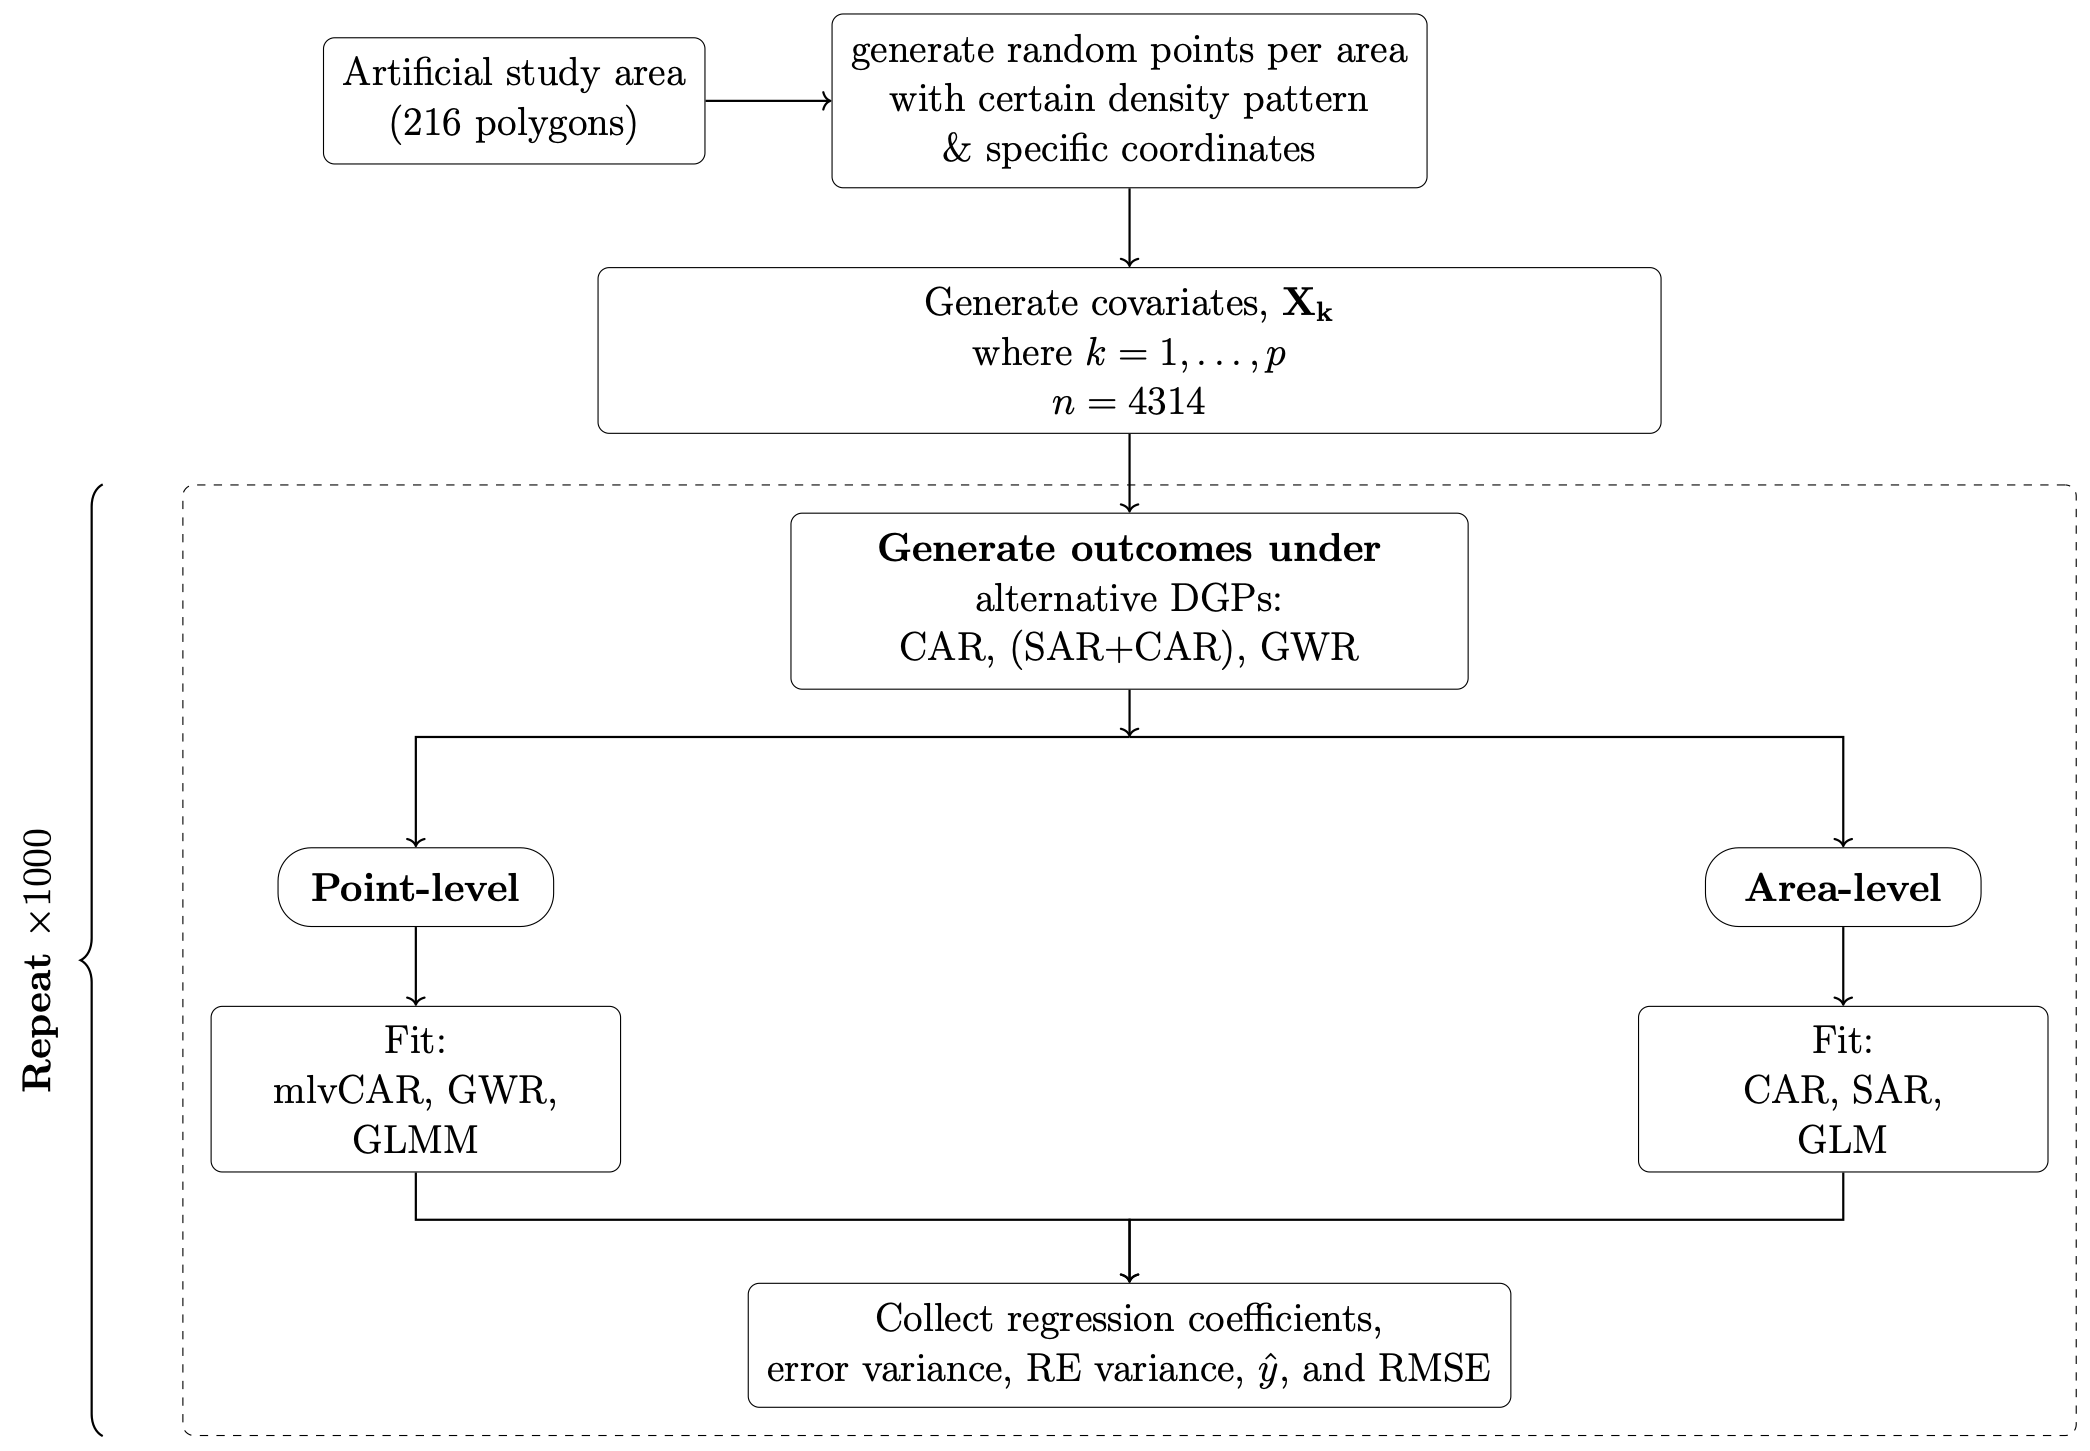
\includegraphics[width=0.8\textwidth]{../figures/experimentdesign0.png}

}

\caption{\label{fig-exp0}Proposed simulation framework. Spatial data are generated under multiple mechanisms (GWR, CAR, and SAR+CAR) and represented at both areal and point levels. A range of competing models is fitted to each dataset, and their performance is systematically evaluated across repeated simulations using bias and RMSE.}

\end{figure}%

\vspace{1.5cc}

\subsection{Artificial Study Region}\label{artificial-study-region}
The experiment begins with the construction of an artificial spatial
region consisting of 216 polygons, each representing a distinct areal
unit. We draw \(K=216\) seed points uniformly inside a Lombok bounding
window (WGS 84
\footnote{World Geodetic System, a global standard for measuring locations on Earth.};
\([116.0^\circ,\,116.5^\circ]\mathrm{E},\,[8.5^\circ,\,8.0^\circ]\mathrm{S}\))
and apply a
\textbf{Voronoi}\footnote{A spatial partition where each region consists of all points closer to one seed than to any other}
tessellation to obtain an irregular lattice \cite{okabe2009spatial}. The
tessellation is then clipped to the window, small sliver cells are
removed using a minimum--area rule, and the result is stored as an
\texttt{sf} layer with CRS EPSG:4326.
\footnote{Coordinate reference system - European petroleum survey group. It is a coordinate reference system defined by an EPSG code, such as EPSG:4326 for WGS 84.}
This yields an areal partition of 216 polygons with realistic variation
in size and number of neighbours.

A map of the final lattice and its neighbourhood graph is shown in
Figure~\ref{fig-artfreg} and serves as the fixed spatial support for all
simulations.

\begin{figure}[H]

\centering{

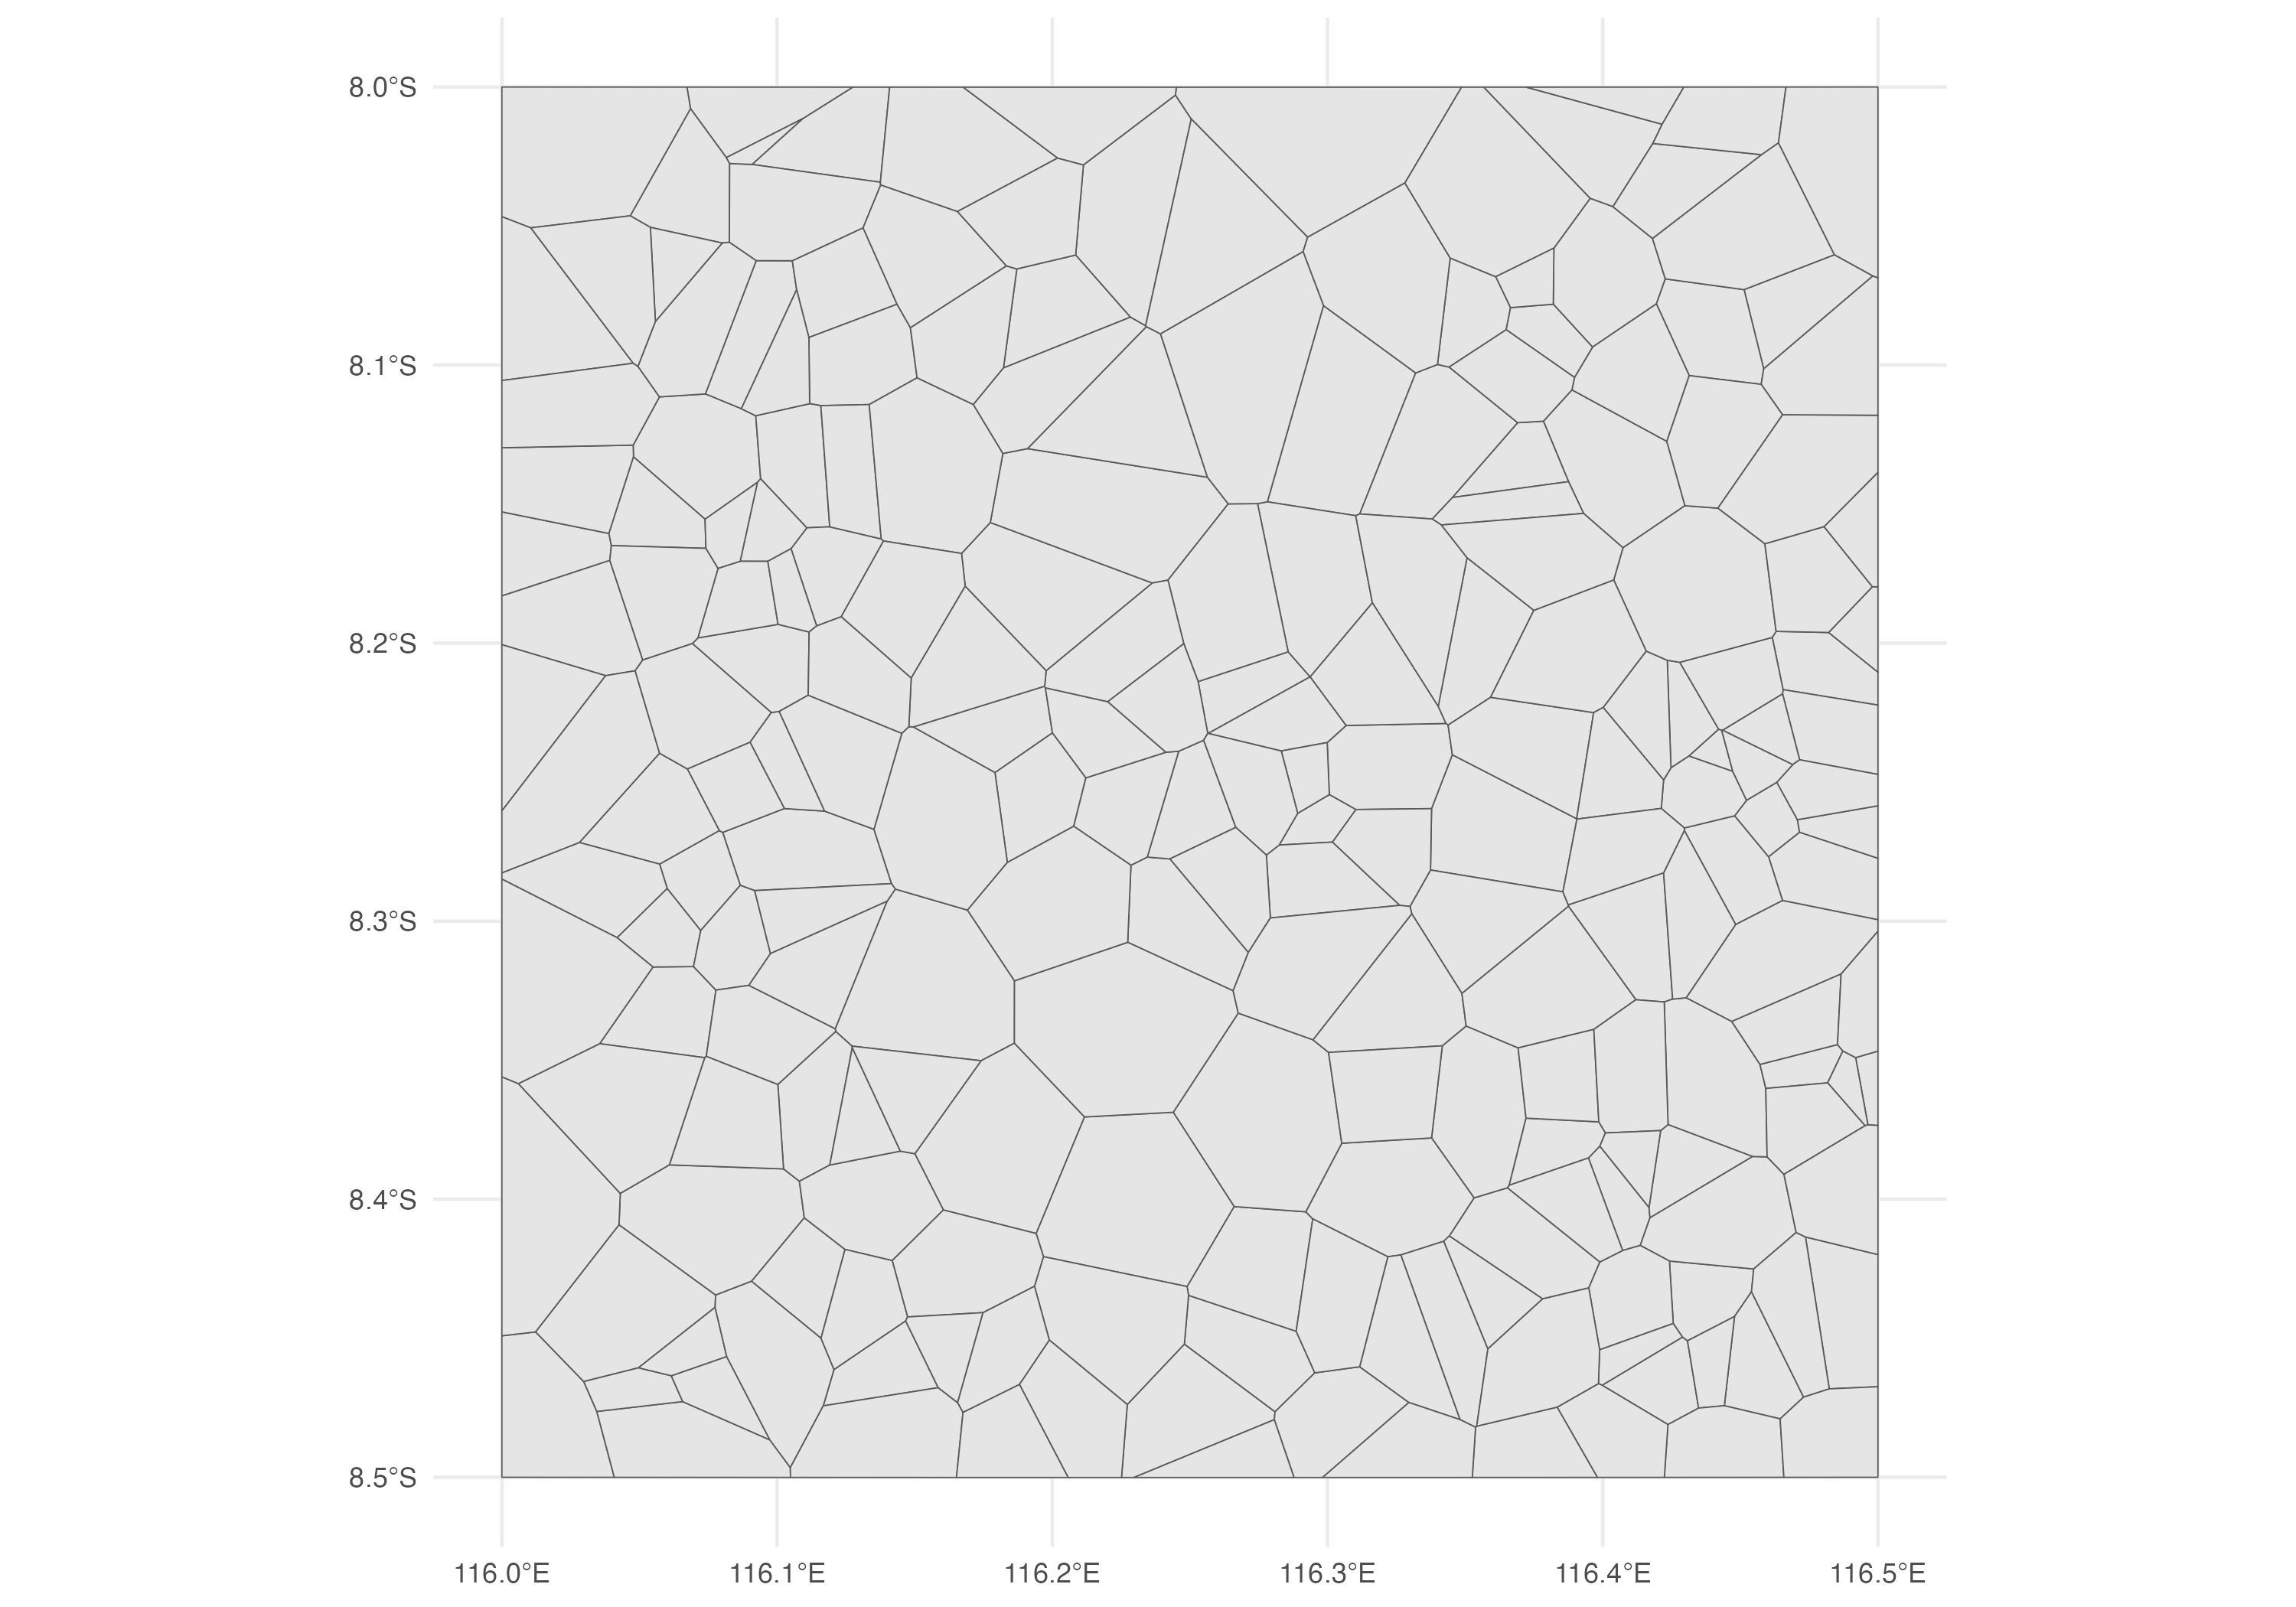
\includegraphics[width=0.9\textwidth]{../figures/artfcountry_plot.png}

}

\caption{\label{fig-artfreg}Artificial areal partition (216 units).
Voronoi polygons clipped to a bounding box; grey lines show polygon
boundaries.}

\end{figure}%

The resulting neighbour graph for the artificial region is shown in
Figure~\ref{fig-neighartfreg}. Edges connect polygons that are
neighbours, providing a visual summary of the
spatial connectivity that underlies the simulations.

\begin{figure}[H]

\centering{

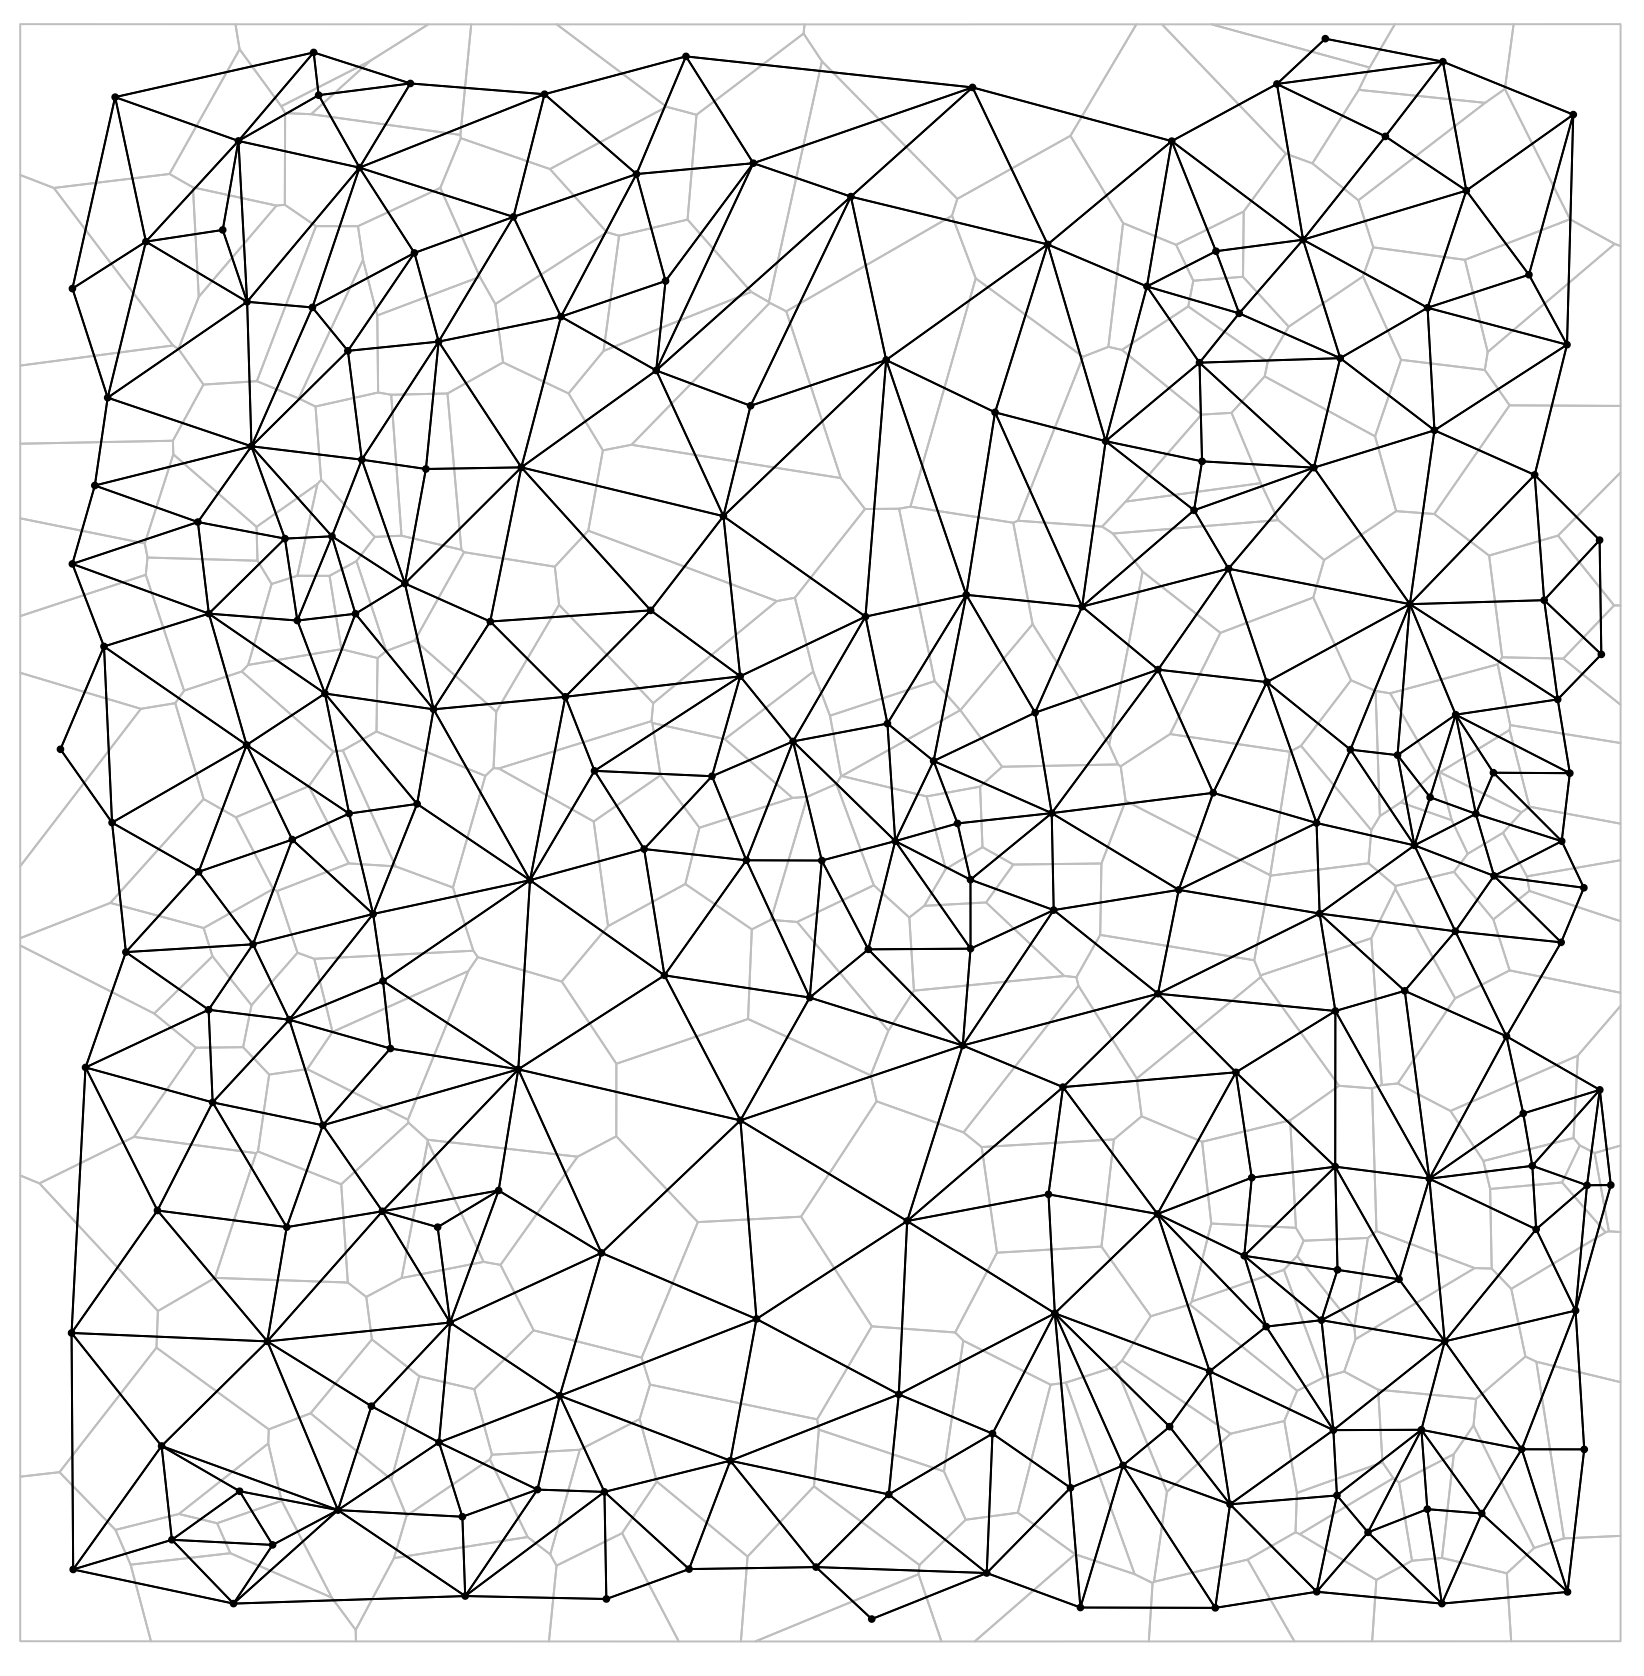
\includegraphics[width=0.6\textwidth]{../figures/nb_artfcountry.png}

}

\caption{\label{fig-neighartfreg}Neighbourhood structure of the
artificial region. This figure illustrates the spatial connectivity
between polygons in the artificial study region, where each line
represents a defined neighbour relationship based on spatial adjacency}

\end{figure}%

\subsection{Synthetic density and point
generation}\label{synthetic-density-and-point-generation}

To emulate realistic spatial variation, the artificial region is endowed
with a density pattern in which a central horizontal belt exhibits
higher housing density, an abstraction inspired by Lombok's population
and development gradient. Density is not used as a covariate in
subsequent models; instead, it controls how many observation points each
polygon receives.

Let \(y_i\) be the \(y\)-coordinate of the centroid of area \(i\). We
define a smooth ridge centered at \(\bar y\) with Gaussian decay and
mild noise, \[
d_i^\star \;=\; \exp\!\left\{-\frac{(y_i-\bar y)^2}{2\sigma^2}\right\} \;+\; \varepsilon_i,
\qquad \varepsilon_i \sim \mathcal N(0,\sigma_\varepsilon^2),
\] truncate below a small floor, and rescale to \([500,1000]\): \[
d_i \;=\; 500 \;+\; 500\,\frac{d_i^\star-\min(d^\star)}{\max(d^\star)-\min(d^\star)} \;\in\; [500,1000].
\]

For each area \(i\), the number of point locations is a bounded affine
function of \(d_i\),

\[
n_i \;=\; \mathrm{clip}\!\left\{\;\Big\lfloor m_{\min}
+ s\,(m_{\max}-m_{\min})\,\frac{d_i-500}{1000}\Big\rceil,\; m_{\min},\; m_{\max}\right\},
\]

with \(m_{\min}=5\), \(m_{\max}=150\), and scaling factor \(s=0.7\).
Points are then sampled uniformly within each polygon. In practice, this
yields \(4{,}314\) points across \textbf{216} polygons, with
\textbf{5--56} points per polygon, reflecting higher concentration in
the central belt. Figure~\ref{fig-pointsonmap} shows the resulting
point-level distribution.

\begin{figure}

\centering{

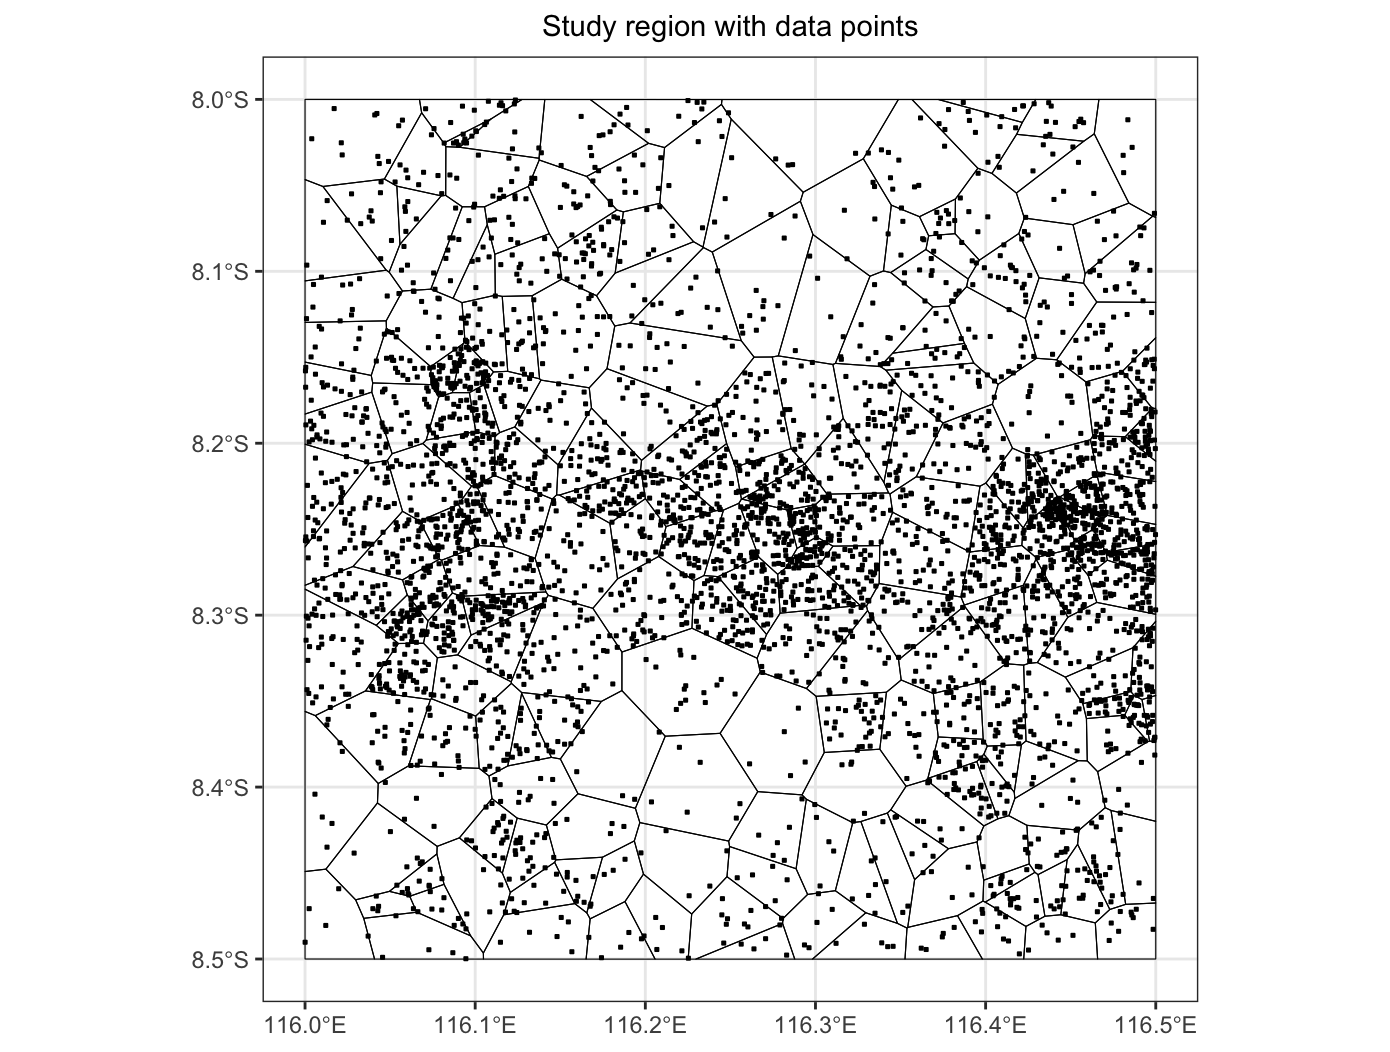
\includegraphics[width=0.8\textwidth]{../figures/density_points_plot.png}

}

\caption{\label{fig-pointsonmap}Artificial study region with observation
points. The points represent data locations within each polygon,
simulating real-world spatial observations for the purpose of model
analysis and validation.}

\end{figure}%

In practice, polygons with higher density yield more observations,
mimicking the fact that densely populated urban centres typically host
more housing transactions. A total of 4,314 points were generated across
the 216 polygons, with each polygon containing between 5 and 56
observations. Figure~\ref{fig-pointsonmap} depicts this
point-level distribution.

\subsection{Covariate Generation}\label{covariate-generation}

Each observation point is assigned four structural attributes used as
explanatory variables for prices: land size (\(X_1\)), building size
(\(X_2\)), bedrooms (\(X_3\)), and bathrooms (\(X_4\)). To induce
realistic co-movement, the point-level vector
\(\mathbf{X}_i=(X_{i1},X_{i2},X_{i3},X_{i4})^\top\) is drawn from a
multivariate normal distribution:

\[
\mathbf{X}_i \sim \mathcal N_4(\,\boldsymbol\mu,\;\boldsymbol\Sigma\,), 
\qquad 
\boldsymbol\mu = (300,\,120,\,3,\,2)^\top .
\]

The covariance is built from standard deviations \(\{50,\,30,\,1,\,1\}\)
and a target correlation matrix \(\mathbf R\) (e.g., \(\rho_{12}=0.8\),
\(\rho_{13}=0.5\), \(\rho_{23}=0.6\), \(\rho_{34}=0.7\)):

\[
\boldsymbol\Sigma = \mathbf D\,\mathbf R\,\mathbf D ,
\qquad \mathbf D=\operatorname{diag}(50,\,30,\,1,\,1).
\]

Draws are mapped to plausible ranges: \(X_1\in[100,1500]\) m\(^2\),
\(X_2\in[40,800]\) m\(^2\), \(X_3\in\{1,\dots,5\}\), and
\(X_4\in\{1,\dots,3\}\) (by rounding and truncation). A representative
slice is shown in Table Table~\ref{tbl-covrstr}.

For areal analyses, point-level covariates are averaged within polygons:

\[
\bar X_{Aj} \;=\; \frac{1}{n_A}\sum_{i\in A} X_{ij}, \qquad j=1,\ldots,4,
\]

where \(A\) indexes polygons and \(n_A\) is the number of points in
polygon \(A\). As a diagnostic, Moran's I (\(1000\) permutations) is
computed on these area-level means to gauge residual spatial
autocorrelation introduced by aggregation.

A representative slice of this dataset is shown in
Table~\ref{tbl-covrstr}.

\begingroup\fontsize{9}{11}\selectfont

\begin{longtable}[t]{lllll}

\caption{\label{tbl-covrstr}Slice of generated dataset as covariates for
simulations}

\tabularnewline

\toprule
ID & Land size & Building size & Bedrooms & Bathrooms\\
\midrule
1 & 270.48 & 108.55 & 4 & 2\\
1 & 295.99 & 100.13 & 4 & 2\\
2 & 319.52 & 126.31 & 3 & 1\\
2 & 325.01 & 120.84 & 4 & 3\\
2 & 294.15 & 144.05 & 4 & 3\\
\addlinespace
3 & 222.18 & 81.4 & 3 & 2\\
4 & 414.23 & 150.15 & 2 & 2\\
4 & 278.75 & 101.41 & 2 & 1\\
$\vdots$ & $\vdots$ & $\vdots$ & $\vdots$ & $\vdots$\\
\bottomrule

\end{longtable}

\endgroup{}

\subsection{Generating Y: Three different DGPs}\label{generating-y-three-different-s}

Given the covariates \(\mathbf X\) and the artificial areal lattice, we
simulate the response \(Y\) under three spatial DGPs: CAR,
SAR+CAR, and GWR. All three data-generating processes
use the same covariate standardisation, neighbourhood support, and
output construction.

For point \(j\) in area \(a\) and covariate \(k\in\{1,2,3,4\}\), \[
X_{ajk}^{\text{std}} \;=\; \frac{X_{ajk} - \bar X_k}{s_k},
\] where \(\bar X_k\) and \(s_k\) are the global mean and standard
deviation computed over all points. The point-level design vector
includes an intercept, \[
\mathbf x_{aj} \;=\; \big(1,\;X_{aj1}^{\text{std}},\;X_{aj2}^{\text{std}},\;X_{aj3}^{\text{std}},\;X_{aj4}^{\text{std}}\big)^\top .
\]

The artificial lattice and polygon contiguity are fixed across scenarios
(Figure~\ref{fig-neighartfreg}). The binary adjacency matrix is
\(\mathbf W\) with diagonal matrix \(\mathbf D=\mathrm{diag}(d_{aa})\),
\(d_{aa}=\sum_b w_{ab}\).

Coefficient values are calibrated from a beta function that is inspired
from GWR concept about spatially varying coefficients as a
function of location coordinate, where in this context it refer to areas
centroid \((x_a, y_a)\), with components specified as
trigonometric--linear trends plus small Gaussian noise
(Equation~\ref{eq-betas})

\begin{equation}\phantomsection\label{eq-betas}{
\beta_k(\mathbf s_a)
\;=\;
b_k
\;+\; c_{k1}\,\sin(dx_a)
\;+\; c_{k2}\,\cos(dy_a)
\;+\; c_{k3}\,x_a
\;+\; c_{k4}\,y_a
\;+\; \varepsilon_k ,
}\end{equation}

The \(sine–cosine\) terms create smooth, oscillating spatial patterns,
the linear terms impose gentle large-scale gradients, and the small
Gaussian perturbations \(\varepsilon_k\) add local variability while
keeping the surfaces smooth (smaller variance for \(\beta_3,\beta_4\)
yields tighter fields for room counts). Evaluating these functions at
polygon centroids yields area-specific coefficients that vary
continuously across the map but remain constant within each polygon,
which is consistent with the GWR design used in the simulations.
values in Equation~\ref{eq-params} are the mean column of beta matrix.
it yields:

\begin{equation}\phantomsection\label{eq-params}{
\boldsymbol{\beta}=(1,\;0.9,\;0.7,\;0.5,\;0.3)^\top,\qquad
\sigma_\varepsilon^2=0.2,\qquad
\sigma_\phi^2=0.6,\qquad
\rho=0.6 .
}\end{equation}

The idiosyncratic noise $\sigma_\varepsilon^2 = 0.2$ and the spatial
variance $\sigma_\phi^2 = 0.6$ imply a spatial-to-nugget variance
ratio of approximately $3{:}1$. This indicates that spatial structure is
clearly present, yet does not dominate the mean signal. The spatial
dependence parameter $\rho = 0.6$ induces moderate smoothing—strong
enough to capture local spillover effects while avoiding numerical
instability near the unit boundary. Using the same parameter set
$(\boldsymbol{\beta}, \sigma_\varepsilon^2, \sigma_\phi^2, \rho)$ for
CAR, SAR+CAR, and GWR ensures that any observed differences are
attributable to the dependence structure rather than differences in
signal strength.

Each scenario constructs a log-scale outcome $\ell_{aj}$, which is then
transformed back to the original scale via
\[
Y_{aj} = \exp(\ell_{aj}).
\]

From each simulated dataset, we export:
\[
\begin{aligned}
\text{Point level:} \quad & \{Y_{aj}, \ell_{aj}, \mathbf{x}_{aj}, a\}, \\
\text{Area level:} \quad & \left\{
\bar{X}_{Ak} = \frac{1}{n_A} \sum_{j \in A} X_{Ajk}, \;
\tilde{Y}_A = \operatorname{median}\{Y_{Aj}\}
\right\}.
\end{aligned}
\]
For comparability, area-level covariates are re-standardised using the
same global $(\bar{X}_k, s_k)$.

\textbf{Scenario 1: GWR DGP (Spatially Varying Coefficients)}

In this scenario, data are generated under the GWR framework, which allows relationships between the
response variable and explanatory variables to vary across space. Unlike
global regression models that assume a constant parameter vector
$\boldsymbol{\beta}$, the GWR model assigns location-specific
coefficients $\boldsymbol{\beta}(\mathbf{s}_i)$ to each spatial point
$i$, enabling local variation in the relationships.

The coefficient surfaces $\boldsymbol{\beta}(\mathbf{s}_i)$ vary
smoothly over space as functions of spatial coordinates $(x_i, y_i)$,
with the addition of small random perturbations to introduce spatial
heterogeneity. The structure follows Equation~\ref{eq-betas}.

Using these locally varying coefficients, the response variable is
generated as
\begin{equation}
\label{eq-gwrgdp}
Y_i = \beta_0(\mathbf{s}_i)
+ \beta_1(\mathbf{s}_i) X_{i1}
+ \beta_2(\mathbf{s}_i) X_{i2}
+ \beta_3(\mathbf{s}_i) X_{i3}
+ \beta_4(\mathbf{s}_i) X_{i4}
+ \varepsilon_i,
\end{equation}
which is derived from Equation~\ref{eq-gwr}, where
$\varepsilon_i \sim \mathcal{N}(0, \sigma_\varepsilon^2)$ represents
independent random noise. This formulation ensures that each observation
reflects a locally adaptive relationship, producing a spatially
heterogeneous dataset suitable for evaluating the ability of GWR to
recover spatially varying coefficients.

\textbf{Scenario 2: CAR DGP (Areal Random Effects)}

Hete, the spatial effect
$\boldsymbol{\phi}$ plays a central role in inducing spatial dependence
among areas. The neighbourhood structure is defined by the spatial
adjacency matrix $\mathbf{W}$, where two areas are considered neighbours
if they share a common boundary.

The spatial random effects $\boldsymbol{\phi}$ are generated from a
multivariate Gaussian distribution following the Leroux prior:
\begin{equation}
\label{eq-lerouxjoint}
\boldsymbol{\phi} \mid \mathbf{W}, \tau^2, \rho, \boldsymbol{\mu}
\sim \mathcal{N}\!\left(
\boldsymbol{\mu},\;
\tau^2 \left[ \rho \mathbf{W}^* + (1 - \rho)\mathbf{I}_n \right]^{-1}
\right),
\end{equation}
where $\mathbf{W}^* = \mathbf{D} - \mathbf{W}$ and $\mathbf{D}$ is a
diagonal matrix containing the number of neighbours for each area. The
matrix $\mathbf{Q} = \rho \mathbf{W}^* + (1 - \rho)\mathbf{I}_n$ acts as
a precision matrix controlling spatial smoothness. Smaller values of
$\rho$ imply weaker spatial dependence, whereas values close to 1
produce stronger spatial autocorrelation.

Once $\boldsymbol{\phi}$ is generated, it is incorporated into the
response according to Equation~\ref{eq-car}, yielding spatially
correlated outcomes that reflect the underlying spatial structure.

\textbf{Scenario 3: SAR + CAR DGP (Lagged Mean and Areal Effects)}

This scenario combines both SAR and CAR structures in a two-stage
process.

In the first stage, the response vector $\mathbf{Y}$ is generated from
its joint distribution, as described in Equation~\ref{eq-jointysar}.
This approach is computationally efficient compared to directly
simulating from the recursive SAR formulation (Equation~\ref{eq-sar}),
where each observation depends on neighbouring values. The covariance
matrix is given by
\[
\sigma^2 (\mathbf{I} - \rho \mathbf{W})^{-1}
(\mathbf{I} - \rho \mathbf{W})^{-T},
\]
where $\rho$ is the spatial autoregressive parameter, $\mathbf{I}$ is
the identity matrix, and $\mathbf{W}$ is the spatial weight matrix.

In the second stage, spatial random effects $\boldsymbol{\phi}$—as
defined in Equation~\ref{eq-lerouxjoint}—are added to the SAR-generated
outcomes:
\[
\mathbf{Y}_{\text{SAR+CAR}} = \mathbf{Y}_{\text{SAR}} + \boldsymbol{\phi}.
\]

This hybrid construction captures both global spatial dependence (via
the SAR component) and localised spatial heterogeneity (via the CAR
component), producing data that more closely resemble complex spatial
processes observed in practice.

\subsection{The Simulations}\label{simulations}

After all simulation components were prepared, the experiments were
conducted in two iterative sets of $M = 1000$ replications. Each set
corresponds to a different level of analysis: point-level and
area-level. The first set (point-level data) involved fitting the
mlvCAR, GLMM, and GWR models. The second set
(area-level data) involved fitting the CAR, SAR, and GLM.

For the GWR model, the fitting procedure requires spatial coordinates
for each observation. Therefore, the coordinates used were the
artificial ones generated during the observation point generation stage
(see Section~2.2). This approach reflects practical constraints in
real-world settings, where it is often difficult to obtain housing
transaction data from web listings that include complete addresses and
precise geographic coordinates.

The CAR and mlvCAR models were estimated using the
\texttt{CARBayes} package, specifically via the functions
\texttt{S.CARleroux} and \texttt{S.CARmultilevel}, which implement
Bayesian inference under the Leroux specification. For the
non-spatial counterparts, the GLMM and GLM models were fitted using the
\texttt{rstanarm} package (\texttt{stan\_glmer}) and the base R function
\texttt{glm}, respectively. This allows for a direct comparison between
spatial and conventional hierarchical modelling approaches. Spatial
dependence based on lag structures and spatially varying relationships
was captured using the SAR and GWR models, implemented via
\texttt{lagsarlm} and \texttt{gwr}, respectively.

From each simulation, the extracted quantities include the estimated
means of the intercept, regression coefficients, and spatial parameters,
such as $\hat{\rho}$, $\hat{\sigma}^2_{\varepsilon}$, and
$\hat{\sigma}^2_{\phi}$. In addition, the corresponding standard
deviations and confidence intervals were computed. The root mean squared
error (RMSE) was also calculated for each iteration as a complementary
measure of model performance.

The simulation outputs were stored in a structured list object using the
\texttt{furrr} package to enable parallel computation across iterations.
Each simulation run produced a set of outputs, including estimated
parameters, spatial parameters, and prediction errors. These outputs
were combined using the \texttt{do.call()} and \texttt{rbind()} functions
to form unified data frames for subsequent analysis.

Specifically, the main simulation object \texttt{sim\_results}
contains results from all $M = 1000$ iterations. Each element of this
object includes:
\begin{itemize}
\item \texttt{params}: estimated regression coefficients and intercepts,
\item \texttt{params\_sp}: spatial parameters such as $\hat{\rho}$,
$\hat{\sigma}^2_{\varepsilon}$, and $\hat{\sigma}^2_{\phi}$, and
\item \texttt{rmses}: RMSE values for model performance evaluation.
\end{itemize}

These components were subsequently extracted and consolidated into three
separate data frames, namely \texttt{params\_df},
\texttt{paramssp\_df}, and \texttt{rmse\_df}, representing the
regression estimates, spatial parameters, and predictive performance
metrics, respectively.

\section{Results}\label{results}

This section presents the outcomes of the simulation experiments,
focusing on the comparative performance of the considered models under
different spatial data-generating processes. The analysis evaluates both
estimation accuracy and predictive capability across point-level and
area-level datasets. In particular, attention is given to the behaviour
of regression coefficients, the magnitude of bias, and overall model fit
as measured by predictive error. The results are organised into two main
components: (i) bias and predictive performance, and (ii) the behaviour
of the spatial dependence parameter $\rho$ across scenarios.

\subsection{Bias and Predictive Performance}\label{bias-and-power-prediction}

Figures~\ref{fig-biaspt} and~\ref{fig-biasar} present the bias estimates
of regression coefficients across different modelling approaches.

Under the CAR data-generating process (DGP), all three models exhibit
relatively low bias, indicating that each is capable of recovering the
true parameter values with reasonable accuracy. However, their levels of
uncertainty differ substantially. The GWR model displays the widest
confidence intervals, reflecting its limited ability to capture the
discrete areal dependence inherent in the CAR process. In contrast, both
the GLMM and mlvCAR models produce tighter confidence bands and more
stable estimates. In particular, the mlvCAR model aligns closely with the
data-generating mechanism, as it explicitly incorporates hierarchical
areal effects similar to those in the CAR structure. This suggests that
models designed to represent spatial random effects yield more efficient
and reliable estimates when the underlying process follows an areal
random-effect structure.

\begin{figure}[H]
\centering
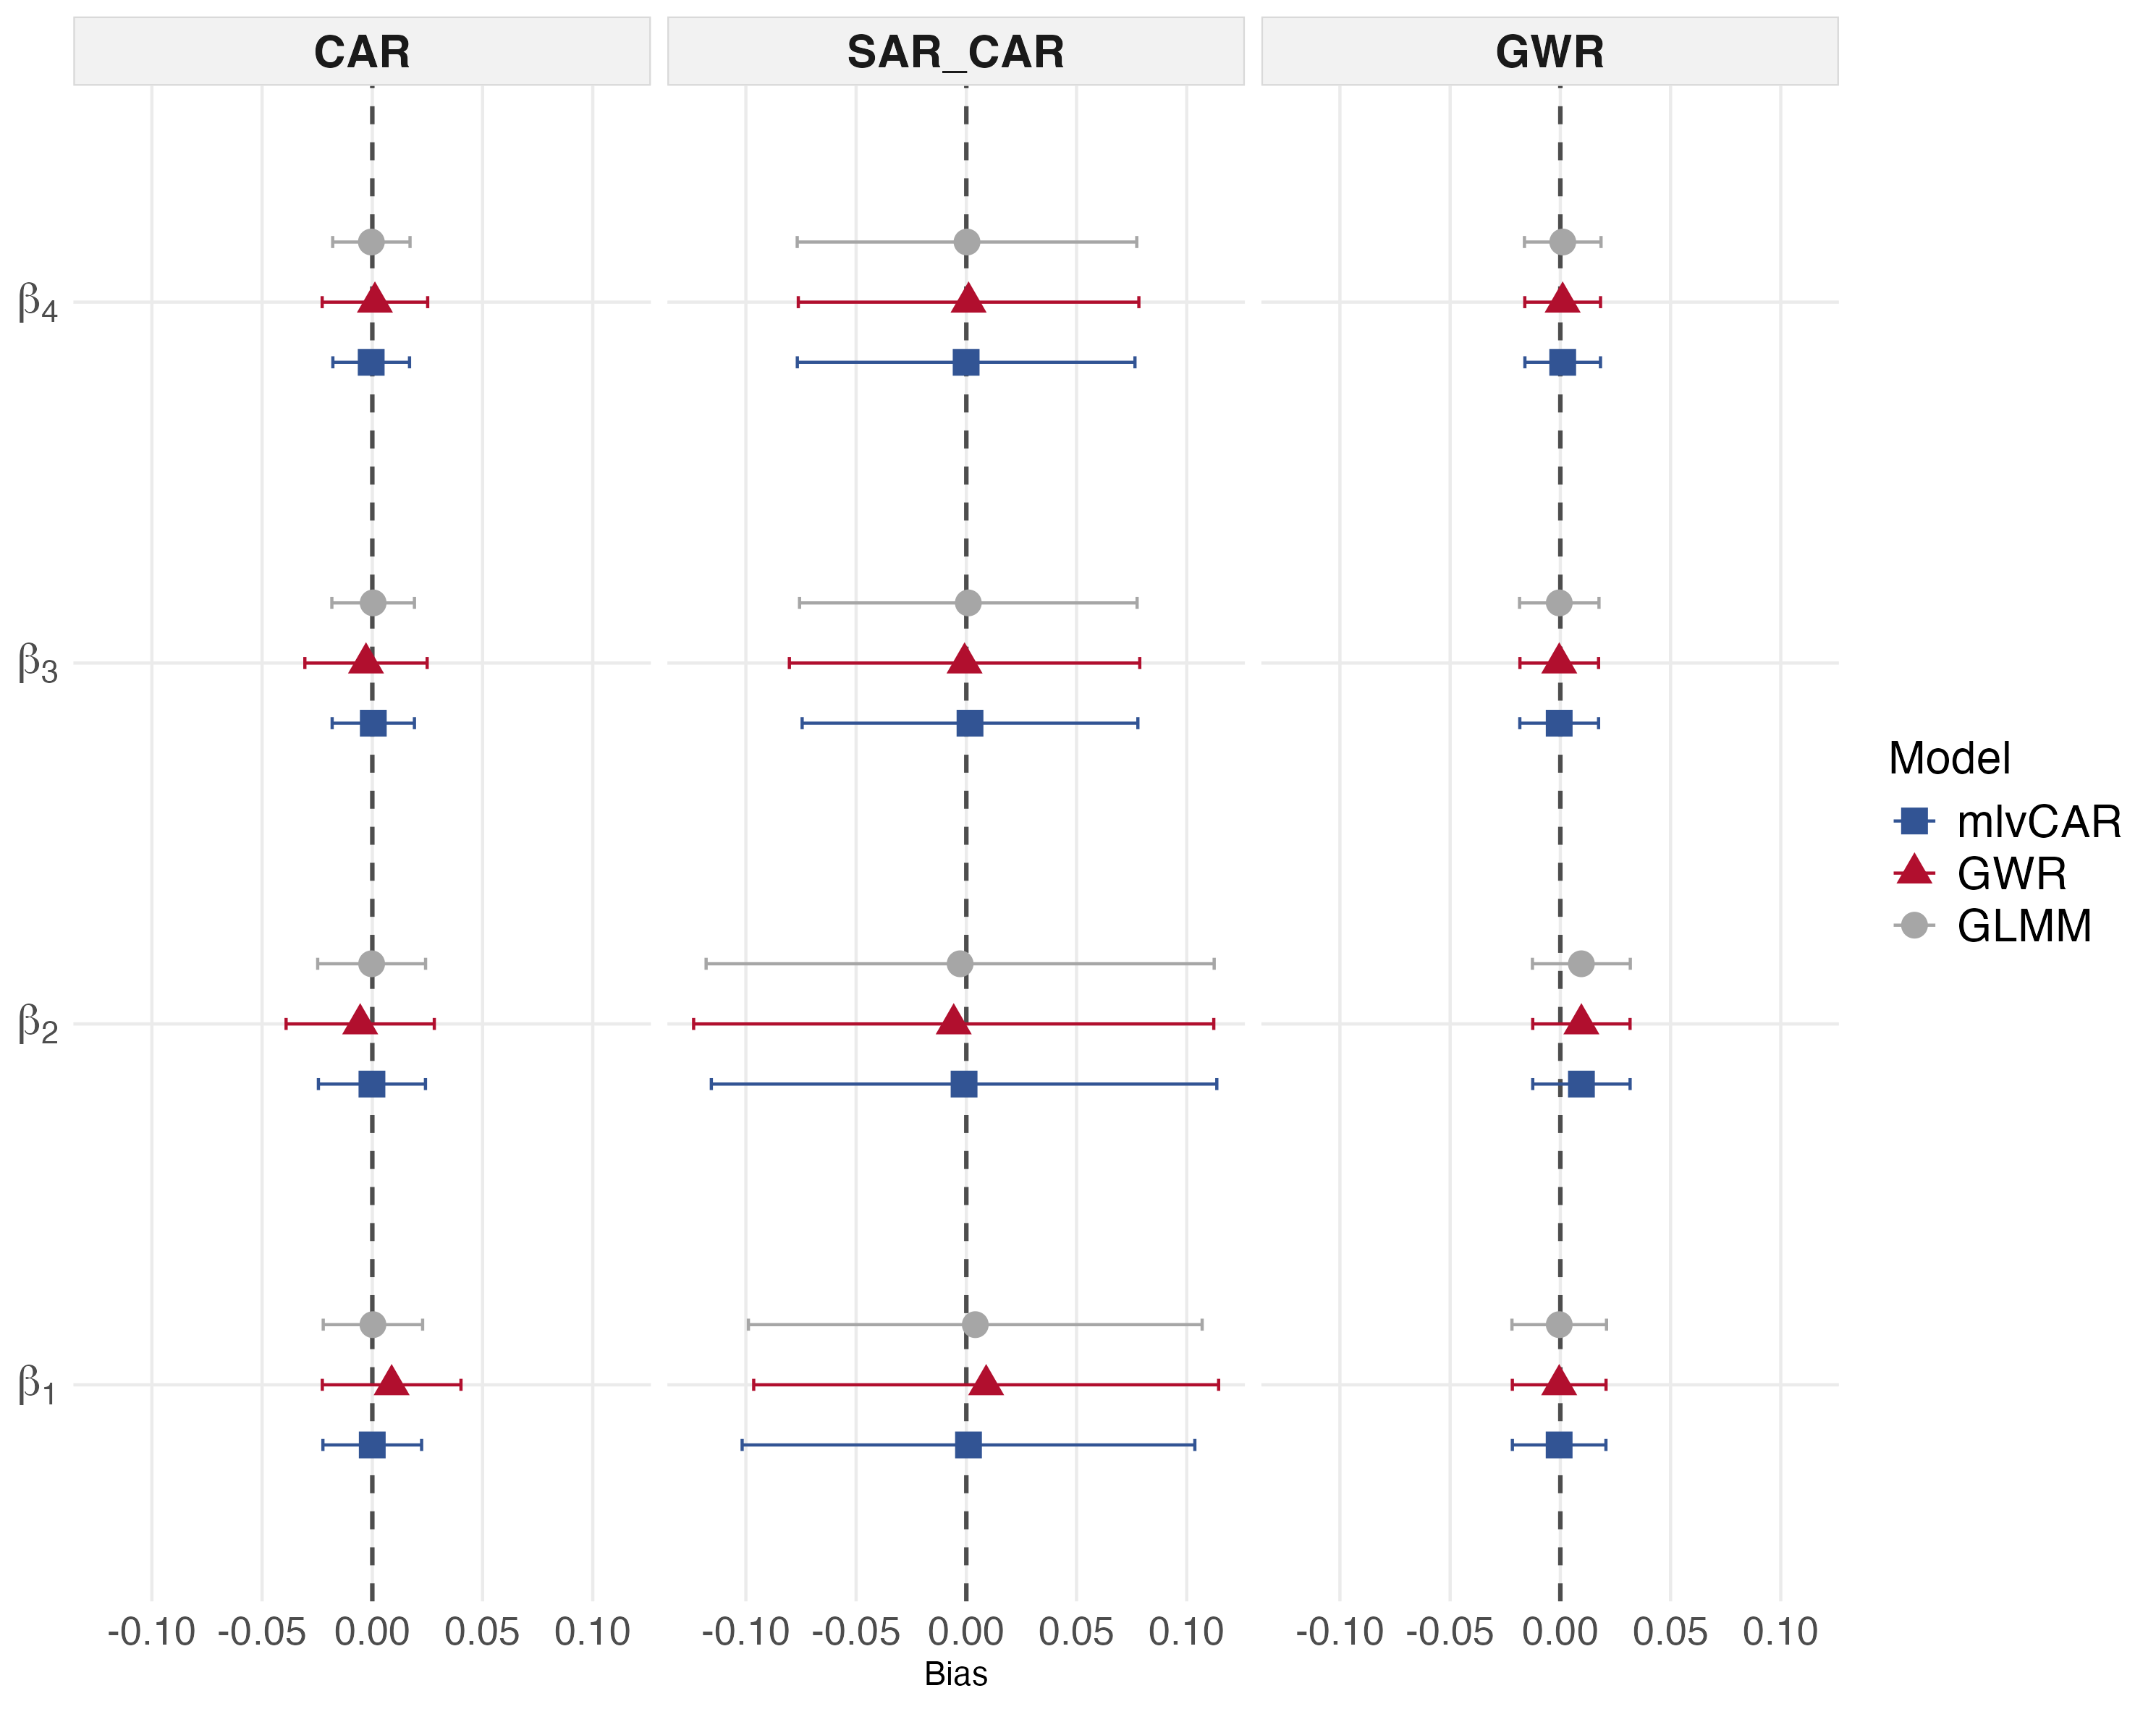
\includegraphics[width=0.85\textwidth]{../figures/bias_point.png}
\caption{\label{fig-biaspt}Bias values by method and dataset type for point-level data}
\end{figure}

Under the SAR+CAR DGP, which combines spatial lag dependence with areal
random effects, all models exhibit increased variability and bias
compared to the previous scenario, reflecting the higher complexity of
the underlying spatial process. The mlvCAR model tends to produce the
most stable estimates, although with wider uncertainty bands, indicating
that it captures areal correlation effectively but does not fully
represent the lag dependence component. The GWR and GLMM models show
greater bias and wider intervals, particularly for coefficients related
to building and land size, highlighting their limitations in modelling
joint spatial lag and random-effect structures. This scenario
underscores the challenges associated with hybrid spatial dependencies
and the need for models that explicitly integrate both components.

When data are generated under the GWR DGP, where spatial variation is
expressed through smoothly varying local relationships, the GWR model
performs as expected, yielding the smallest bias and narrowest
confidence intervals across all coefficients. This confirms its
effectiveness in capturing continuous spatial heterogeneity. The GLMM
also produces relatively unbiased estimates, albeit with slightly larger
dispersion, as it does not explicitly account for spatial dependence. In
contrast, the mlvCAR model remains stable and largely unbiased but shows
broader uncertainty than GWR, reflecting its approximation of continuous
variation using discrete areal random effects. Nevertheless, mlvCAR
performs robustly, indicating that hierarchical spatial structures can
partially capture smooth spatial variation.

For the area-level datasets, bias patterns remain generally small across
all models, suggesting that each approach is capable of recovering the
true parameters with reasonable accuracy. However, distinct differences
emerge depending on the underlying DGP.

Under the CAR DGP, the CAR, GLM, and SAR models all produce nearly
unbiased estimates, with values centred around zero and relatively
narrow confidence intervals. The CAR model performs best in this
setting, as expected, due to its direct alignment with the underlying
areal dependence structure. The GLM and SAR models also provide stable
estimates, although the SAR model exhibits slightly greater variability,
likely due to its lag-based formulation.

Under the GWR DGP, bias remains close to zero across all models,
indicating robustness even when the true process follows continuous
spatial variation. However, confidence intervals are slightly wider,
particularly for the SAR model, reflecting structural mismatch between
the assumed and true processes.

\begin{figure}[H]
\centering
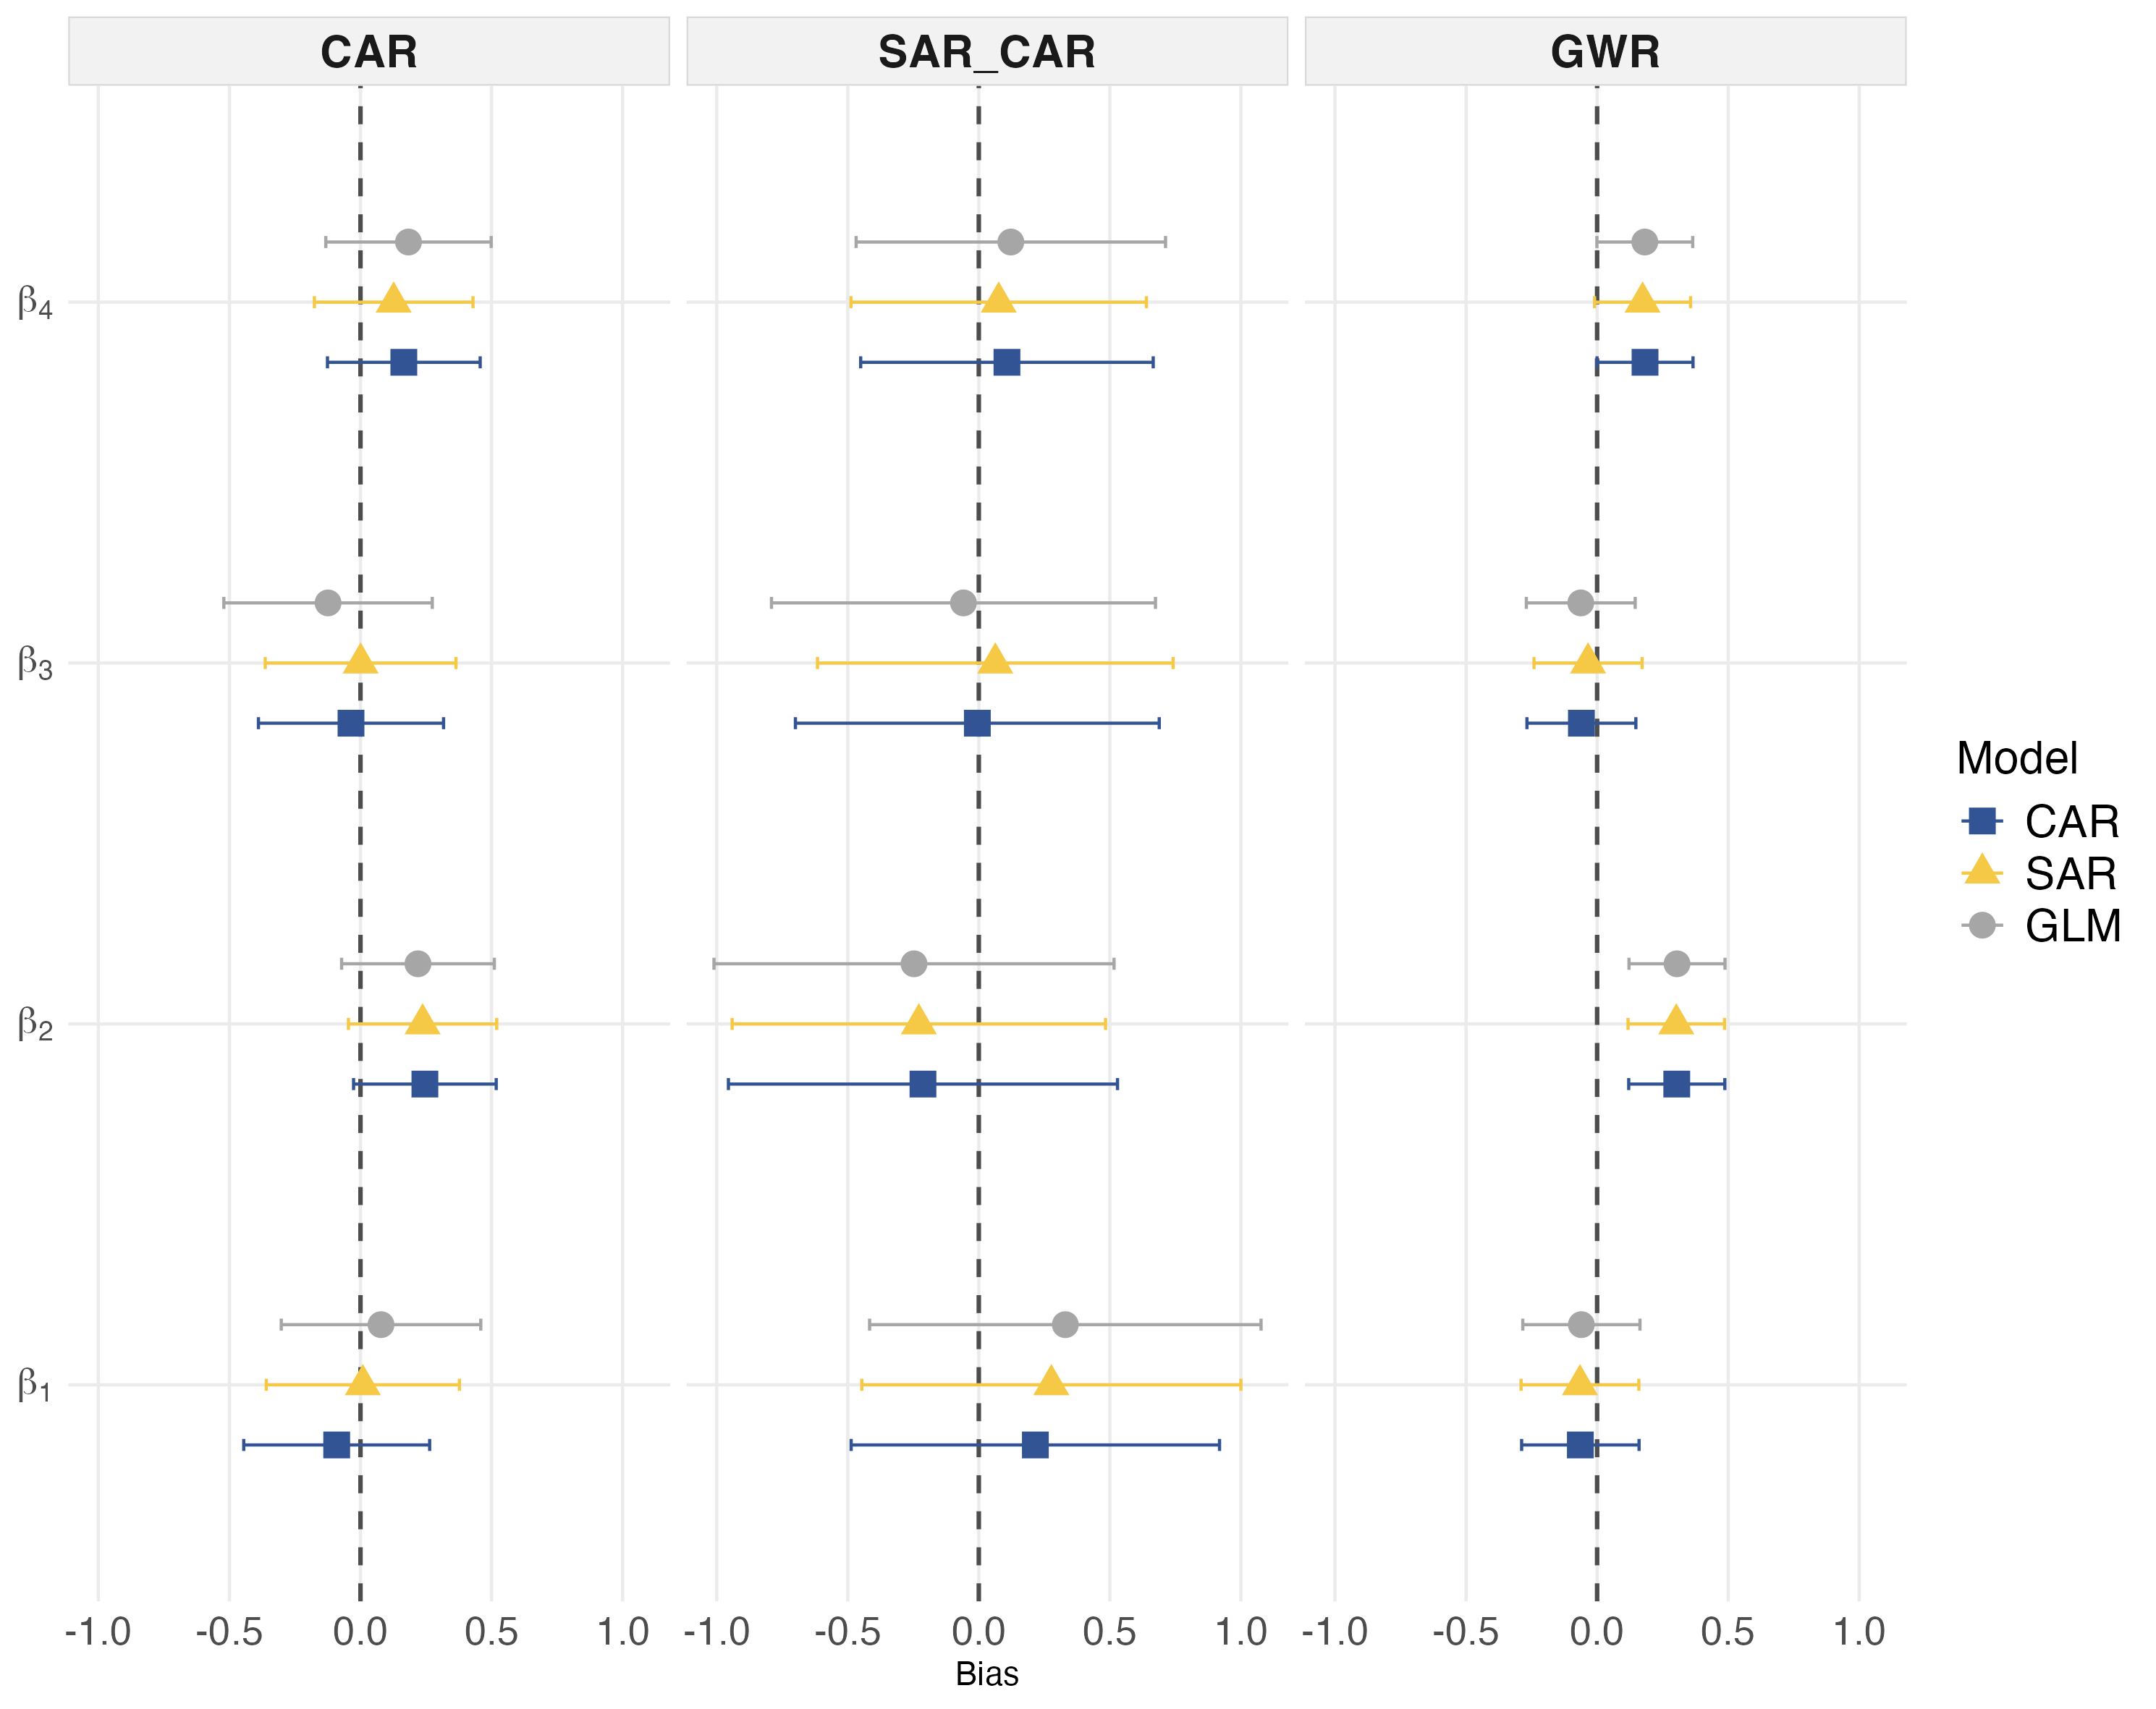
\includegraphics[width=0.85\textwidth]{../figures/bias_area.png}
\caption{\label{fig-biasar}Bias values by method and dataset type for area-level data}
\end{figure}

In contrast, the SAR+CAR DGP produces the largest variation among
models. The SAR model remains relatively unbiased but shows higher
uncertainty, benefiting from its ability to capture lag dependence. The
CAR model performs consistently, although its confidence intervals widen
slightly due to the added complexity. The GLM, lacking an explicit
spatial component, exhibits greater bias and variability, highlighting
its limitations in modelling spatial dependence.

Overall, these results indicate that the CAR model performs most
reliably when spatial dependence is driven by areal structures, while
the SAR model provides advantages under mixed dependence settings. The
GLM yields stable but spatially naïve estimates, performing adequately
only when spatial dependence is weak or absent.

% \begingroup
% \fontsize{9}{11}\selectfont
% 
% \begin{longtable}{lrrrrrr}
% \caption{\label{tbl-rmse}RMSE values across different datasets} \\
% 
% \toprule
% \multicolumn{1}{c}{} & \multicolumn{3}{c}{Area-level data} & \multicolumn{3}{c}{Point-level data} \\
% \cmidrule(l{3pt}r{3pt}){2-4} \cmidrule(l{3pt}r{3pt}){5-7}
% Dataset & GLM & SAR & CAR & GLMM & GWR & mlvCAR \\
% \midrule
% \endfirsthead
% 
% \toprule
% \multicolumn{1}{c}{} & \multicolumn{3}{c}{Area-level data} & \multicolumn{3}{c}{Point-level data} \\
% \cmidrule(l{3pt}r{3pt}){2-4} \cmidrule(l{3pt}r{3pt}){5-7}
% Dataset & GLM & SAR & CAR & GLMM & GWR & mlvCAR \\
% \midrule
% \endhead
% 
% \bottomrule
% \endfoot
% 
% \bottomrule
% \endlastfoot
% 
% CAR & 4.09 & 3.85 & 1.81 & 14.04 & 21.13 & 9.94 \\
% SAR+CAR & 11.88 & 11.68 & 3.88 & 47.67 & 48.87 & 38.97 \\
% GWR & 2.43 & 2.42 & 2.28 & 18.31 & 18.33 & 14.87 \\
% 
% \end{longtable}
% \endgroup

\begin{figure}[H]
\centering
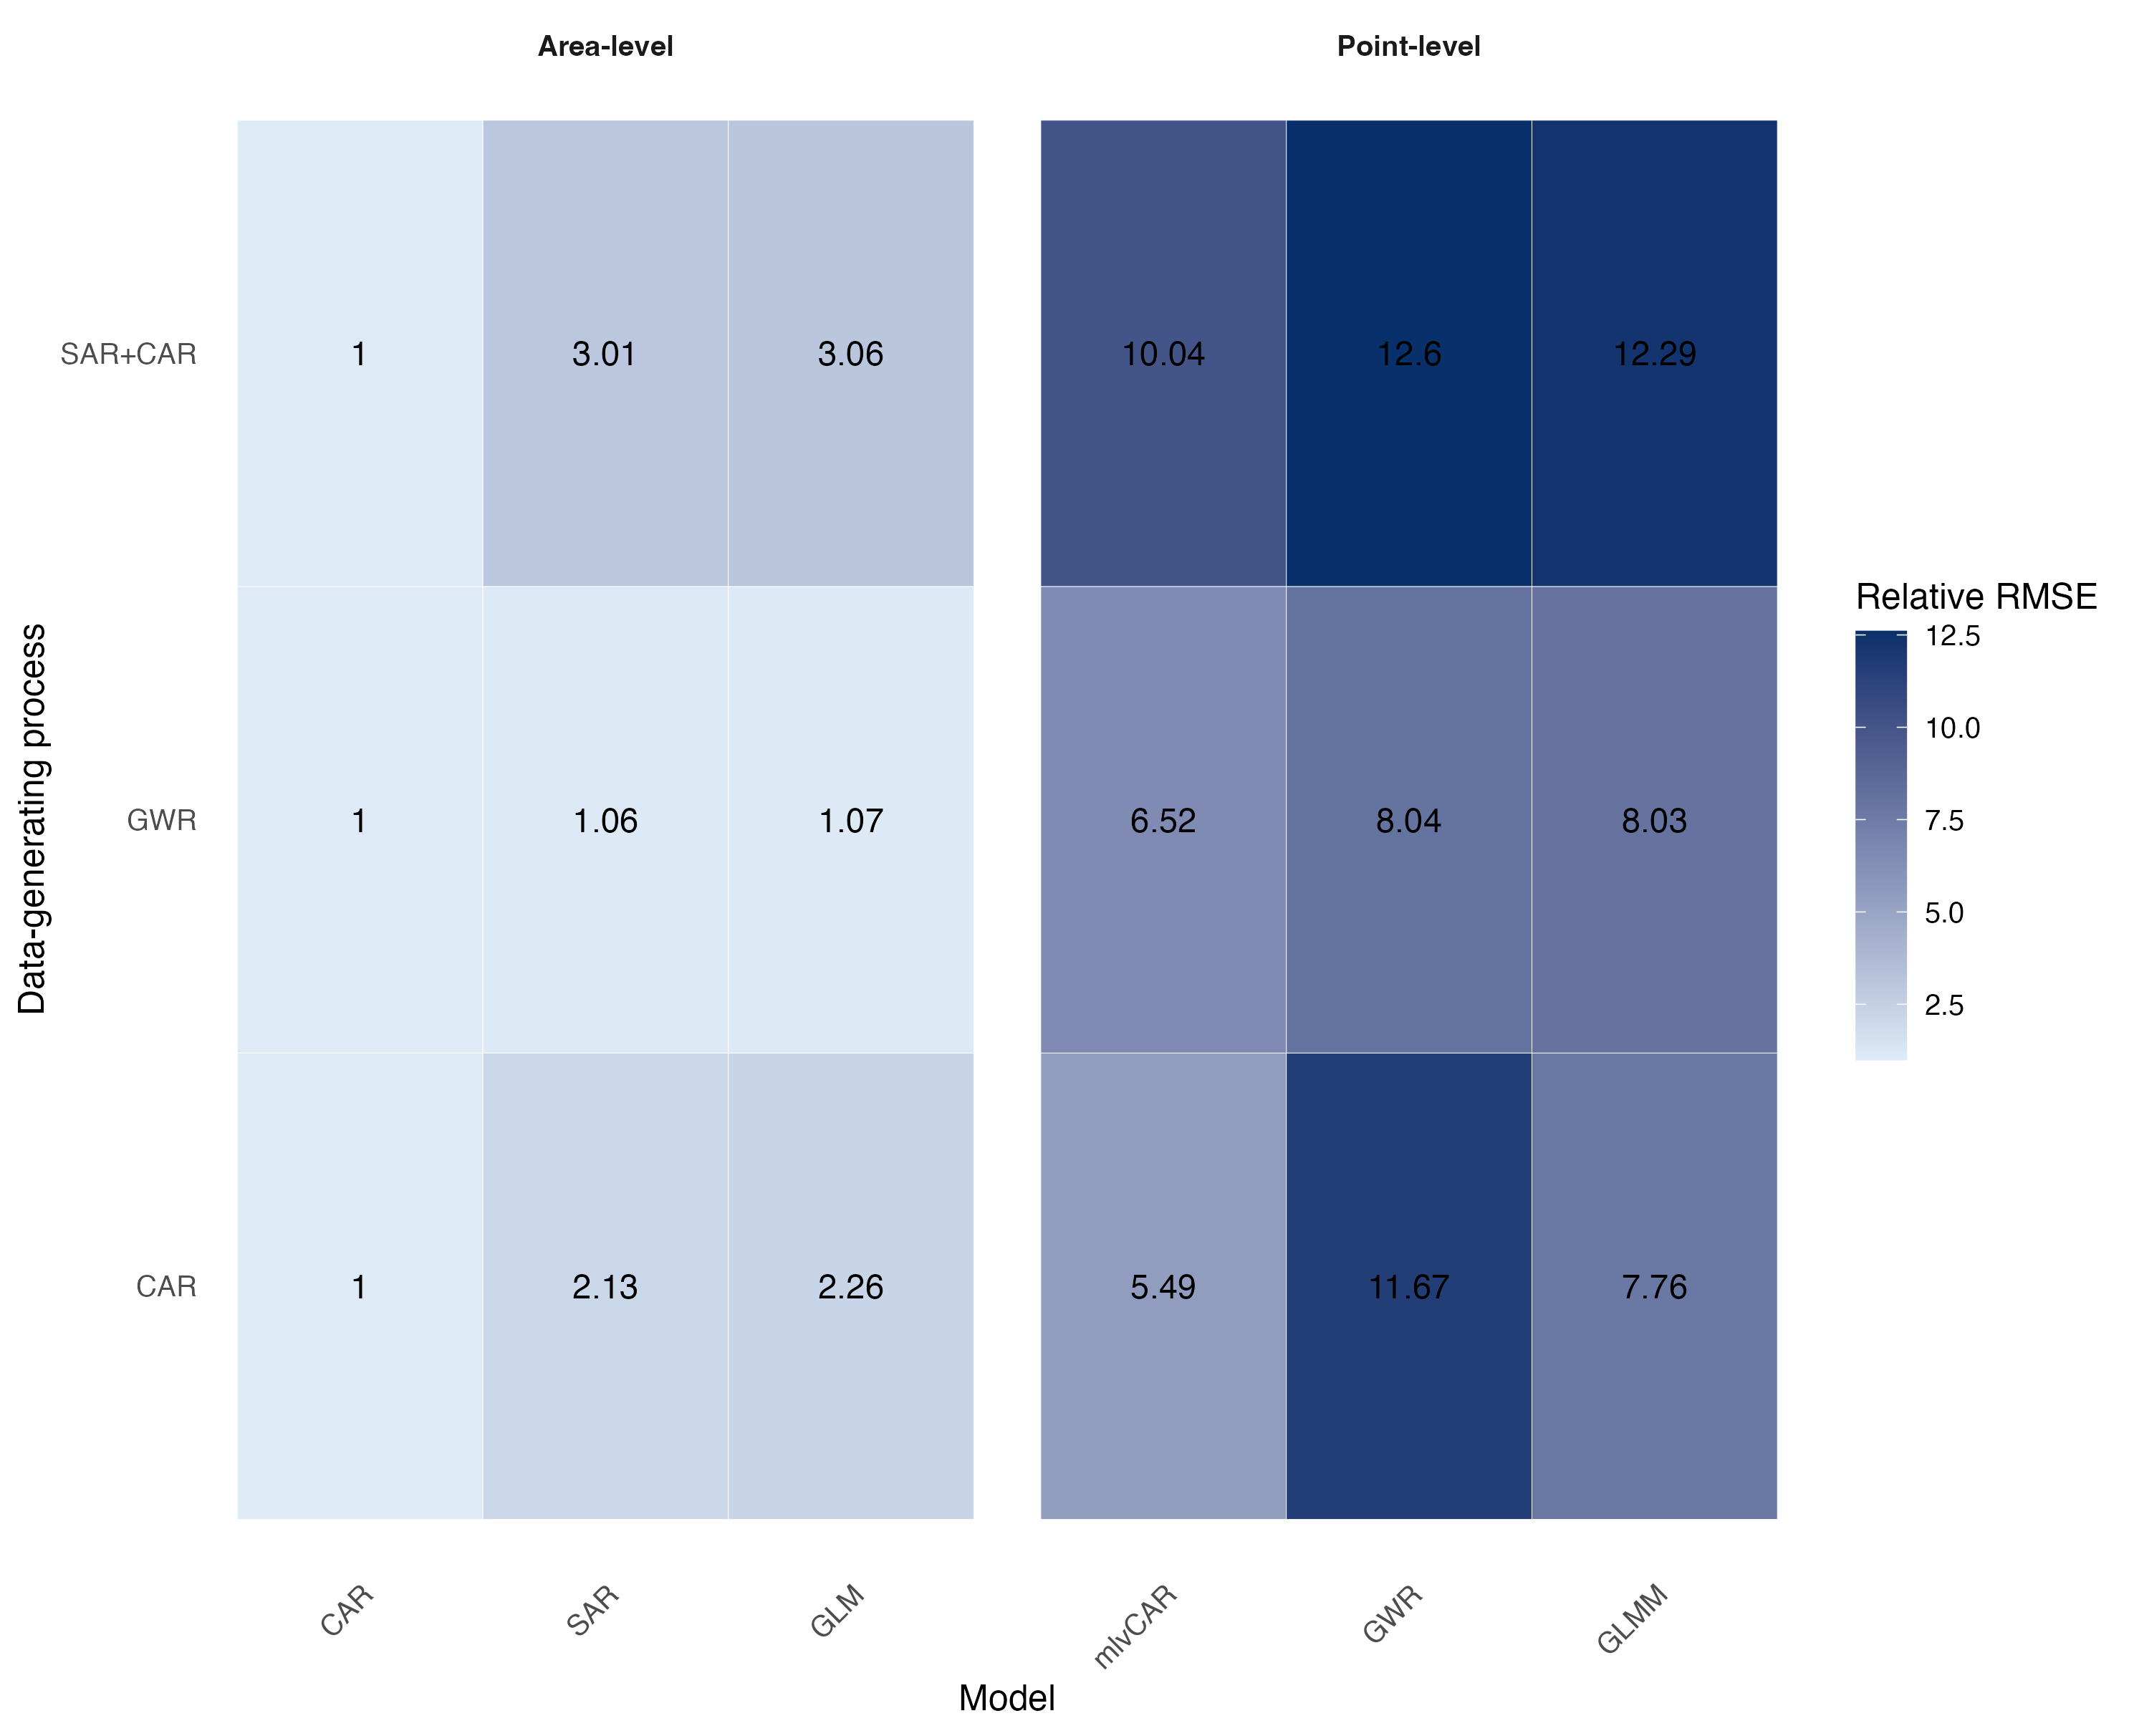
\includegraphics[width=0.85\textwidth]{../figures/rmseplot.png}
\caption{\label{fig-rmse}Heatmap of relative RMSE for competing models under different spatial data-generating processes. Results are shown for both areal and point-level data, with values normalised within each scenario (lower values indicate better performance).}
\end{figure}


Figure~\ref{fig-rmse} presents relative RMSE heatmap for all models under three
data-generating processes, evaluated separately
for area-level and point-level datasets. Lower RMSE values indicate
better predictive performance.

For the area-level data, the CAR model consistently exhibits the best performance across all data-generating processes, as indicated by the lowest relative RMSE in each scenario. This confirms its strong suitability when spatial dependence is primarily driven by areal random effects. Under the CAR DGP, the CAR model clearly outperforms both GLM and SAR, while under the SAR+CAR DGP it remains the most accurate, indicating robustness to more complex spatial structures. In contrast, under the GWR DGP, all models show comparable relative performance, suggesting only limited loss in accuracy when the true spatial process is continuous rather than discrete.

For the point-level data, the mlvCAR model demonstrates the strongest overall performance, achieving the lowest relative RMSE across all scenarios. Its advantage is evident under both the CAR and SAR+CAR DGPs, where it consistently outperforms GLMM and GWR. Although all models experience a degradation in performance under the GWR DGP, the mlvCAR model remains the most stable, indicating greater robustness to different forms of spatial dependence. Overall, these results highlight the benefit of incorporating hierarchical spatial structure when modelling point-level data.

Overall, these findings suggest that:
\begin{itemize}
\item CAR-based models (CAR and mlvCAR) are most effective when spatial
dependence arises from areal or hierarchical structures;
\item the SAR model performs moderately well but does not outperform CAR;
\item GWR and GLMM are less effective in the presence of discrete or
mixed spatial dependence;
\item CAR (area-level) and mlvCAR (point-level) emerge as the most
reliable models across varying spatial data structures.
\end{itemize}

\subsection{Insights from $\rho$ Values Across Data Scenarios}

Figure~\ref{fig-rho} illustrates the distribution of the estimated
spatial autocorrelation parameter ($\rho$) across the three
data-generating scenarios (CAR, SAR+CAR, and GWR). Each boxplot
summarises results from 1000 simulation replications. Note that only
three models—CAR, mlvCAR, and SAR—include the spatial dependence
parameter $\rho$.

The CAR model consistently produces high $\rho$ estimates, with median
values around $0.6$--$0.7$, particularly under the CAR DGP. This confirms
its effectiveness in capturing areal spatial dependence.

\begin{figure}[H]
\centering
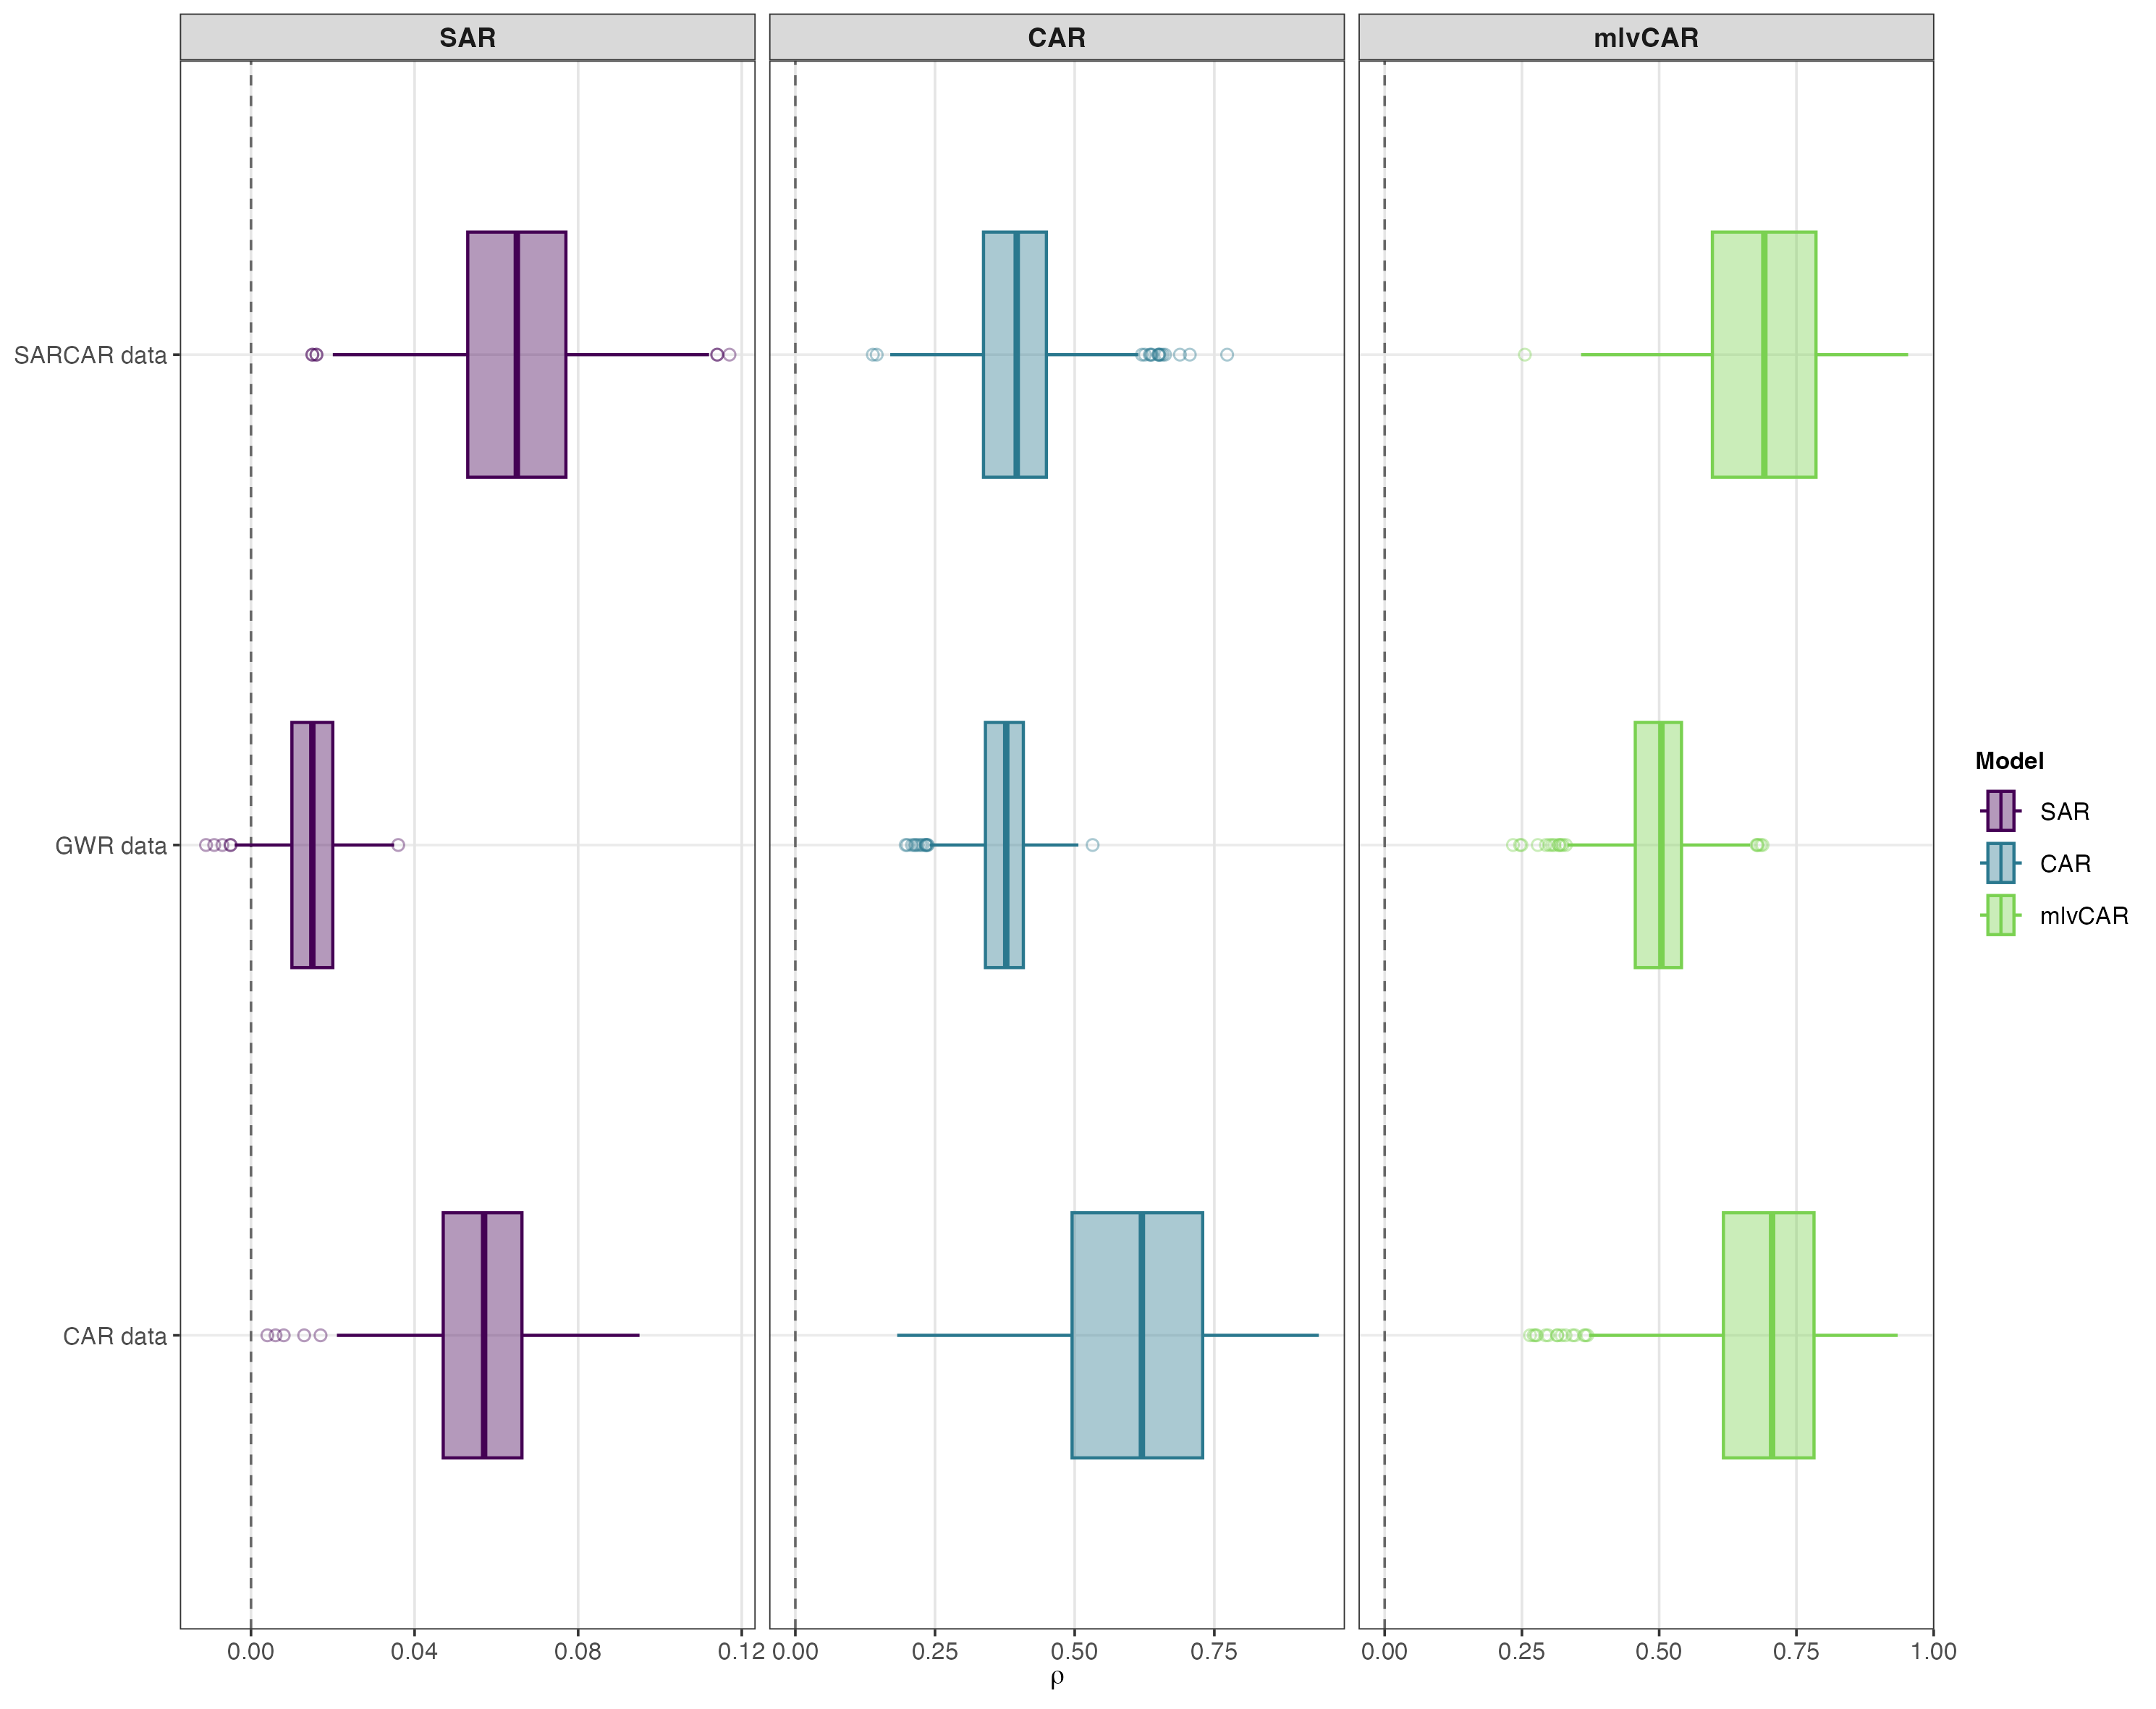
\includegraphics[width=1\textwidth]{../figures/rhos.png}
\caption{\label{fig-rho}Distribution of $\rho$ estimates across models and scenarios}
\end{figure}

The mlvCAR model exhibits a similar pattern but with a wider spread of
$\rho$ values, reflecting its hierarchical structure that captures both
within- and between-area dependence. This additional flexibility allows
it to accommodate more complex spatial relationships.

In contrast, the SAR model yields substantially lower $\rho$ estimates,
indicating that lag-based dependence is less suited for areal data where
correlation arises from shared boundaries. Interestingly, even under the
GWR DGP, both CAR and mlvCAR detect meaningful spatial dependence,
suggesting that adjacency-based models can partially capture smooth
spatial variation, albeit in an aggregated form.

The results highlight the importance of aligning the modelling framework with the underlying spatial structure of the data. Models that correctly reflect the data-generating process, such as CAR for areal data and mlvCAR for point-level data, consistently achieve the best performance. However, the findings also demonstrate that certain models exhibit greater robustness to misspecification. In particular, the mlvCAR model maintains relatively stable performance across all scenarios, suggesting that hierarchical spatial formulations provide a flexible framework when the true spatial mechanism is unknown.

Furthermore, the comparison between area-level and point-level analyses underscores the impact of data aggregation. The loss of spatial detail at the areal level can lead to different model behaviour and performance, reinforcing the importance of considering data resolution in spatial modelling. From a practical perspective, these results suggest that while simpler models such as CAR remain effective for areal data, more flexible hierarchical approaches are advantageous for point-referenced data and in situations where spatial structure is complex or uncertain.

\vspace{1.5cc}

\noindent \textbf{Data Availability Statement}. The data used to support the findings of this study are available from the corresponding author upon request.

\vspace{1.5cc}
\noindent \textbf{Declarations}. A conflict of interest, also known as a competing interest, is a situation in which an interest or connection -direct or indirect-could influence your research.   

\vspace{1.5cc}
\noindent \textbf{Author Contributions}. 
% \noindent \href{https://www.elsevier.com/researcher/author/policies-and-guidelines/credit-author-statement}{CRediT} (Contributor Roles Taxonomy) Authorship Contribution statement is introduced to recognize individual author contributions, reduce authorship disputes, and facilitate collaboration. CRediT allows author to share an accurate and detailed description of their diverse contribution to the published work. The corresponding author is responsible for ensuring that the descriptions are accurate and agreeable by all authors. The role(s) of all authors should be listed using the relevant above categories. Authors may have contributed in multiple roles. Credit in no way changes the journal’s criteria to quality for authorship. CrediT statement should be provided during the submission process.
% 
% \noindent \noindent \textbf{Possible CRediT statements}:
% Conceptualization, data curation, formal analysis, funding acquisition, investigation, methodology, project administration, resources, software, supervision, validation, visualization, writing-original draft, writing-review \& editing.

% \noindent \textbf{Sample CRediT author statement}:
Indira Puteri Kinasih: Conceptualization, writing-original draft, visualization, software, validation. Haziq Jamil: Conceptualization, methodology, Data curation, formal analysis, resources, writing-review \& editing, data curation. Elvynna Leong: writing-review \& editing, methodology. 

\vspace{1.5cc}
\noindent \textbf{Funding Statement}. This research received no specific grant   343from any funding agency in the public, commercial, or not-for-profit sectors.

\vspace{1.5cc}
\noindent \textbf{Acknowledgment}. If there are any, write the acknowledgment or appreciation in this section. Acknowledgments can be addressed to those individuals, institutions, and laboratories who provided help during the research (e.g., providing language help, writing assistance or proof reading the article, reviewers, etc.). It could be also to people who contributed to the article or data in the article (excluding the authors).

%Below is the list of references that are cited in the text. Do not include any paper that are not cited in the text. Make sure that the details are correct.

\vspace{2cc}

\bibliographystyle{ieeetr}
\bibliography{../refs}

\end{document}
